\documentclass[UTF8,a4paper,8pt]{ctexbook} 

\usepackage{graphicx}%学习插入图
\usepackage{verbatim}%学习注释多行
\usepackage{booktabs}%表格
\usepackage{geometry}%图片
\usepackage{amsmath} 
\usepackage{amssymb}
\usepackage{listings}%代码
\usepackage{xcolor}  %颜色
\usepackage{enumitem}%列表格式
\CTEXsetup[format+={\flushleft}]{section}
\geometry{left=1.6cm,right=1.8cm,top=2cm,bottom=1.7cm} %设置文章宽度
\pagestyle{plain} 		  %设置页面布局
\author{郑华}
\title{2016 Diary}



\begin{document} 		 %正文排版开始
 	\maketitle
   
 \section*{January}
 
 
 
	 \paragraph{Day 1   Friday   \quad   晴天}
	 
		 Hello,HUA:
		 
		 新年的第一天留给了同学的婚礼。
		 
		 认识了一个叫麻静的妹子,
		 
		 压了门,要了红包,挡了路
		 
		 晚上到宾馆睡了觉。
		 
		 学会了一个叫 狼人的游戏。
	 \paragraph{Day 2   Saturday    \quad     晴天 \quad 8:40}
		 Hello, HUA:
		 
		 早上,跳跳蛇请坐车回来,然后世斌请着吃了饭我就一路颠簸回学校。
	    
		 晚上回来放松了会儿。
	    
	     新的一年对于自己才刚刚开始。
	 
	 \paragraph{Day 3   Sunday      \quad    晴天  \quad 9:30 }
		 Hello,HUA:
		 
		 早上看着手表,让时间定格到9点然后起床
		 
		 来到办公室着手复习组合数学
		 
		 10:30 开了组会,知道了范玉玲同学是在看论文,找点子的方式进行写论文
		 
		 明确了 利用Maya 进行3D人物建模的开端
		 
		 定制了近期的软件著作权的工作计划
		 
		 然后中午拿着美丽姐的卡高高兴兴的到上岛吃牛排去了
		 
		 下午回来剪了头发,洗了澡,在宿舍待到18:00吃了饭,然后来到实验室继续学习,但是学习效率并不是想象中的那样一直高效。
		 
		 所以适当的休息是特别必要的。
		 
		 明天就要考组合数学了,感觉其实挺有用的,但是就是没学好,但也希望能过吧。
	 \paragraph{Day 4   Monday      \quad    晴天 \quad  7:40 }
	 
		 Hello,HUA:
	 
		 考试终于完了。
		 
		 下午学习了一下午c++
	 
		 然后看了下LaTex 
	 
		 晚上玩了一晚上游戏
	 \paragraph{Day 5   Tuesday     \quad   霾 \quad  12:00  }
	 
		 今天可以说玩了一天
	 
		 早上,存宝他们叫着吃了饭
		 
		 晚上跟着李嵩出去去了次酒吧,这是真的酒吧唉
	 
		 回来玩了会儿游戏,就这样结束了一天
	 \paragraph{Day 6   Wednesday   \quad     }
	 \paragraph{Day 7   Thursday    \quad    灰 \quad  12:00 }
		 Hello,HUA:
	 
		 不知道怎么了,渐渐失去了学习和前进的动力.
		 
		 制定的时间表一个也没实现。反而陷入拖延的境界
		 
		 看了书,并没有总结
		 
		 以任务为记录而非时间,这种模式试试
		 
		 I Can
	 \paragraph{Day 8   FRIday    \quad    HUI \quad 12:00 }
	 
		 丢失了,迷失了。
	 \paragraph{Day 9   Saturday  \quad    12:00 }
		 迷失,继续自责中
	 \paragraph{Day 10  Sunday \quad  12:00   \quad   晴朗与混天到底现在没区别了}
	 
		 Hello,HUA:
		 
		 终于知道 时间是怎么 溜走的了,正如《因为痛,所以叫青春》上所说-“现在最让学生上瘾的应该是网上冲浪和网络游戏。为了在日后回顾走过的青春岁月时不留下悔恨的眼泪,请减少或戒掉这些活动,特别是游戏吧,它们对你的未来毫无益处”
		 
		 今天同往常一样(这周),12:00起来,然后玩一天游戏(Tanks)
		 
		 回顾起来,是夹杂着自责的活着。
		 
		 \subparagraph{周记 \quad 18周截}
		 这周就是玩了一周游戏,没什么进展
     \paragraph{Day 11  Monday   \quad     12:00  \quad 灰}
     
	     Hello,HUA:
	     
	     想走出低迷吗? 如果你真的想如此,其实比想象的要简单。  关键在于 将时间周期弄得短一些,没错,就是解决好“今天”的事情就行。
	     
	     你只要踩好今天的第一脚就可以满足了。无数个“今天”会以惊人的速度集合起来,让勤奋集合成惯性。
	     
	     今天被老范问了一个很当头炮的问题“如果老妈和老婆同时掉水,你会 救谁?”
	     
	     我的回答是“在老妈身体已经不行的情况下救老婆,在适当条件下我也犹豫了半天”
	     
	     我的判定是,既然愿意抛出这个为难的问题问我,那我也没必要对她还抱有一丝幻想,有时就是一句话可能就不会再和你聊1句话。
	     
	     这他妈的我凭什么要回答她呢?
	     
	     今天晚上上课被老师批评了,感觉其实批评的确实也在理,希望以后做事能靠谱点,给人一份信任感
	     
	     
     \paragraph{Day 12  Tuesday \quad  10:30 \quad  雪+冷     }
	     Hello,华仔:
	     
	     今天为了应付这个中特社会主义我也是拼了,但是这么不道德的课程简直无语了。而且还是必修...
	     
	     下午洗了个澡,神清气爽
	     
	     晚上玩了会游戏,火炮要成神$\sim$
     \paragraph{Day 13  Wednesday    \quad   8:00 \quad 还可以  }
     
	     Hello,郑华:
	     
	     今天终于结束了这学期的课程,一种解脱,也是一种失去。
	     
	     下午学了会儿C++ ,发现不学跟技术的差距真的是越来越大了。
	     
	     所以得天天学习,了解了解最新科技。
	     
	     晚上照常玩了一下午。
     \paragraph{Day 14  Thursday    \quad    12:30 }
	     hello:
	     
	     今天下午学习了C++ 的新特性,晚上则玩了一晚上。
     \paragraph{Day 15      \quad     }
     \paragraph{Day 16  Saturday   \quad  晴天}
	     Hello, Today:
	     
	     今天过的是否值得,是否有意义,感觉一天都被玩耍占用了。
	     
	     能不能好好的了。
     \paragraph{Day 17  Sunday   \quad   晴天  }
	     Hello,zhengHua
	     
	     今天跟往常一样也是12:30 起床,然后跟着魏拓出去吃了个饭,下午堕落的玩了一下午游戏,晚上一起出去吃了煎饼,晚上跟他们比了CS, 洗了个澡,然后什么也没干。
	     
	     \subparagraph{周记 \quad 19截}
	     
	     玩了一周,也看了看C++11 的一些特性,还不错。只不过是看书的进度没了。
	     
     \paragraph{Day 18  Monday    \quad   晴天  }
     
	     Hello,Hua
	     
	     下午他们约出去玩了CS,就这样下午完了,晚上回来玩了羽毛球,接着做了会儿作业,然后就玩了一晚上游戏。
     \paragraph{Day 19  Tuesday   \quad   干冷     }
	     Hello,Hua
	     
	     今天起床12:40,下午做了会儿作业,玩了会游戏,然后跟着魏拓和存宝吃了烧烤,晚上回来玩了会游戏,把软件体系作业提交了
	     
	     明天要去滑雪了,好激动...
     
     \paragraph{Day 20  Wednesday   \quad    阴 }
     
	     Hello,早上起床结伴而行,滑雪大冒险。好爽,感觉存宝的执行力确实是值得学习的。
	     
	     滑雪还是很有意思的,摔,但摔的很快乐
	     
	     晚上回来的警察狼人游戏也玩的很嗨,谢谢大伙给我这样的日子。
     \paragraph{Day 21  Thursday    \quad    灰 }
	     Hello,HUA:
	     
	     今天又玩了一天游戏。。。
	     
	     中午陪文号下山买了苹果,然后存宝请吃了羊肉泡莫,晚上玩了游戏,顺便巩如悦过生日。
     \paragraph{Day 22  Friday    \quad   HUI  }
	     Hello,ZhengHua
	     
	     早上起床再创记录 2:00,起来后送文浩到咸阳,吃了特香特 泡馍,确实挺香的,晚上回来玩了会游戏
     \paragraph{Day 23  Saturday    \quad   Brisk  }
     
	     Hello,ZhengHUA
	     
	     早上起来晓东走了,被魏拓和存宝叫醒去吃了饭,下午在实验室玩游戏,晚上存宝请着到“什么汉堡”吃了汉堡快餐,好冷啊
     \paragraph{Day 24      \quad     }
     \paragraph{Day 25  Monday    \quad   brisk  }
	     Hello ,zhenghua:
	     
	     今天还是要记录下的, 早上李嵩叫醒了我,起床后用寒冷的冷水洗了头,与他们校门口相见,到东北人家吃了饭,下午k歌,晚上跟存宝和魏拓到小可香再词吃了他们的菜,还是不错的,昨天也是这样的菜,,,
	     
	     明天就要到西安吃喝玩乐了,关键是后天就可以回家了。
     \paragraph{Day 26   To XiAn   \quad  }
	     Hello, Zhenghua:
	     
	     早上10:30 起身去西安,吃了 “麻辣尚席”,特别的辣,特别的爽。
	     
	     下午找到锦城宾馆 住了下来,玩了一晚上扑克。
	     
	     
     \paragraph{Day 27   To Home   \quad     }
	     Hello,ZhengHua:
	     
	     早上10:00  坐上 901 公交去城北客运站,回家的路总算找到了,下午坐上回汉村的车,回来吃了家里土豆丝的味道,晚上同家人一起睡,
	     
     \paragraph{Day 28   vacation 1   \quad     3爸儿子生日}
	     你好,2016年1月28,
	     
	     今天早上起来同学校一般,亦是10点左右,起来后饭后得知  3爸老小过生日,中午随之到镇上吃了饭,饭上也有过错须记,在家中不应主动说饭食不足,而另请加食。
	     
	     中午时候,超超已来了,得知他已经找到工作,在湖北中铁12局。
	     
	     晚上回来开始看电视剧《琅琊榜》
	     
     \paragraph{Day 29   vacation 2   \quad    电视剧 }   
	     你好 2016年1月29日,
	     
	     早上起床已晚,父亲前去参加同学邀请聚会,母亲随同上县去买衣服,家中一人,电视剧又是一天。
	     
     \paragraph{Day 30   vacation 3      \quad  电视剧完   }
	     你好,2016年1月30,
	     
	     早上起的亦晚,随后吃饭
	     
	     下午饭时被母亲批评不孝,不计给家中电话,责备一番。
	     
	     晚上将电视剧看完,将最近事件一一记录。
     \paragraph{Day 31   vacation 4   \quad   腊月22-集市 \quad Sunday }
	     Hello 2016年1月31,
	     
	     今天主要还是以看电视为主要,并没有什么明确性的事件值得记录。
	     \subparagraph{1月记}
	     不知不觉一个月都过去了,然而新年的伊始却没有任何结果,碎碎的时间竟然没有一点值得回顾的价值。生活的意思便渐渐变得淡薄...
	     
	     读书计划又推迟了...不过发现闲暇时间读书也挺快的。《因为痛,所以叫青春》在路上看完了
	     
	     假期本来的计划是好好学习,将DirectX 11 学习到进阶水平,可事实是看了好几天的电影,唉,,,
	     
	     还有这身体情况,一天在床上都不见运动,再这样肌肉都有萎缩了....
	     
	     还有这看书,感觉只是看,看完之后的读书笔记还是需要写的。
	     
	     假期其实也是要有时间表的,本来就与同龄人拉开了差距,他们在努力的工作中积累经验,而我却...
	     
	     假期心中的计划还未明确,而时间并不多了... 
	     
	     为人处事是需要原则的,但是并没有成书,感觉这个得马上写,为人处事为本
	     
	     故,最近事宜:
		 \begin{itemize}[fullwidth,itemindent = 2em]
		  	\item  制定时间表
		 	\item  制定\verb|__|lifePlan
		 	\item  制定假期计划
		 	\item  严格执行
		 \end{itemize} 
		 
		 时间表:
		 \begin{itemize}[fullwidth,itemindent = 2em]
		 	\item  9:00 起床
		 	\item  11:00 开始学习
		 	\item  14:00 午睡
		 	\item  15:00 吃饭
		 	\item  17:00 学习
		 	\item  21:00 休息
		 	\item  23:30 看书
		 	\item  24:00 睡觉
		 \end{itemize}
		 
		 计划:
		 \begin{enumerate}[fullwidth,itemindent = 2em]
		 	\item  C++ basic
		 	\item  C++ 设计模式学会并实现
		 	\item  C++ 数据结构复习并实现一遍
		 	\item  C++ Boost
		 	\item  C++ MFC
		 	\item  C++ cocos2D-x游戏开发过程
		 \end{enumerate}
 
 
 \newpage
 \section*{February}
 
 	 \paragraph{Day 1   vacation 5    \quad  结婚被下书  }
	 	 Hello 2016年2月1日,
	 	 
	 	 今天是2月的第一天,晚上看了IBM的简介,早上却没能起来,中午姑父来下书,而两位老人却没一个拿手机,在家无事实在惭愧,后驱车前去崔叫,
	 	 
	 	 下午则深睡,晚上看电影,最后在睡觉之际看了会儿教学视频。
	 	 
	 	 总的来说,在进步中,还不错...
 	 \paragraph{Day 2   vacation 6    \quad  劳动改造   }
	 	 Hello 2016年2月2,
	 	 
	 	 早上被父亲和母亲的争吵声吵醒,跟着他们到苹果地捡了树枝,好苦...
	 	 
	 	 晚上回来做到床上看着电脑视频,好爽...
	 	 
	 	 差距好大,这就是劳动对人的最大提醒...加油,we Can do that
 	 \paragraph{Day 3   vacation 7     \quad   Home to aware to Book }
 	 \paragraph{Day 4   vacation 8     \quad   Home to sleep  }
	 	 Hello, 2016 year 2 月 4日,
	 	 
	 	 wisdom, justice, fortitude, temperance.
	 	 
	 	 早晨睡觉到 12:00, 如此接近学校的学习.
	 	 
	 	 下午看了会电视剧《Big Bang》
	 	 
	 	 接着睡觉
	 	 
	 	 看了《角斗士》
	 	 
	 	 big Bang...
	 	 
	 	 what the big idea about the C++, what it contains? how to seperate that? and how to use time to learn or re-study..
	 	 
	 	 Never give up. Such strong belief often gives us the second chance. The fact that we fail somewhere does not mean we are going to fail everywhere, and it does not necessarily mean that we are deprived of opportunities to win there. Many successful people did fail before.
	 	 
 	 \paragraph{Day 5   vacation 9    \quad  Learning and clean the clothes}
	 	 Hello 2016年2月5日,
	 	 
	 	 凌晨看了 《岛上书店》的第一章的第一节,刚开始。
	 	 
	 	 起来时,老爸就给我开始忙着弄火炉了...
	 	 
	 	 早上起来学习了会 C++
	 	 
	 	 然后吃了饭,将脏衣服脱下换洗。
	 	 
	 	 下午则荒废了,而老妈在洗衣服...洗衣机坏了,而老妈的手也洗破了..
	 	 
	 	 两个小弟上来陪我,感觉有人陪就是一种不同的感觉吧.
	 	 
	 	 晚上接着看了会儿 C++, 然后看了 The Episodes<反击>
	 	 
	 	 Thinking critically can make one analyze problems insightfully. We live in a world where controversial issues are often simply taken for granted. Critical thinking is but to ask some simple yet essential questions,which always bring amazing outcomes. Thinking Critically can help one comncentrate on right targets. Concentrating on right targets is probably the only way to overcome such dilemmas. Only by thinking critically can one make decisions wise and prudent. Sound decision making is essential to success. By analyzing insightfully and concentrating on the right targets, wise decisions are not hard to reach at all.
	 	 
	 	 认真思考能让人们深入理解问题,做出正确决定。
 	 \paragraph{Day 6   vacation 10   \quad  sleep and clean house somehow}
	 	 Hello,
	 	 
	 	 not do anthing at all, just learn the Enum in C++.
	 	 
	 	 and watch the episodes which name strike back.
 	 \paragraph{Day 7   vacation 11    \quad  除夕}
	 	 Hello, 2016年2月7日||2015年最后一天 阴历||过年,
	 	 
	 	 今天还是一天比较曲折的,早上起来吃饭后,被老爸叫着去祭奠祖坟,这本没什么,可是却偏偏要下去看奶奶,本来看奶奶没什么,就是回家时绕着走了,然后越拖越坏,反而不知该如何下去看望老人家, 下去后,遇到一个不会说话的3妈,一下这场面尴尬的..."研究生来了",然后奶奶接着说“研究生还记着他奶奶啊”,关键这中间爷爷也过来了,抱着3爸的小孩,“看看这些人...”,我竟然不知道该怎么待在这地方
	 	 
	 	 本来说可以缓解尴尬的局面却成了如此境地.
	 	 
	 	 接着2爸帮忙圆了一下话,让我到隔壁叫3爸去上坟,上坟后,我就跟着爸上家贴对联了,问题出在我,总是不愿意配合,也怪老爸,总是在过节时吊着一个脸,然后贴对子恰好碰到OKC VS GSW的第四节的最后一分钟..无巧不成浊,就这弄得这中午一阵怪味。
	 	 
	 	 这件事过去了,接着我坐在门口的小车上晒着太阳看着书,看着“玛雅的成长”让我想到父母陪我长大的记忆..书本本来就是写给某个年龄段的人的,《岛上书店》,我拿了瓶啤酒,一边喝一边看,老爸让我让开,说要用车倒垃圾,这本来就好不容易的安静又被这样打破了,然后是老妈...
	 	 
	 	 中午吃了羊肉面,“huoLuo”,老爸吃了一半听说有打麻将,扔下就走了,我没忍住又多嘴了几句,...
	 	 
	 	 妈也出去了,隔壁没生火的屋就我一个,冷清,看着电视剧,好冷..
	 	 
	 	 中途上了个厕所,23爸的儿子们上来问要红包,本身就不多的零钱哪来的红包啊,自然没给,说是不给,其实心底还是准备给的,可是他们就这样走了,留给我的是一阵失意..原本还准备跟他们打上一晚上的扑克牌呢..
	 	 
	 	 晚上看着美国派时老爸叫下去拜年,我说不去,老爸又来叫了,这次恰好这情节老爸不能看,我把电脑关了,跟着走到主室,说好条件“9点前回来”,走了,下去后,二爸家就奶奶一个,说到2爷家去了,我陪着奶奶,老爸找他们去了,陪到8:15左右我走了,回来老妈给我做了西红柿炒辣椒拌面,麻辣豆腐...一边吃一边看春晚,一边看着微信,这老家的网速真是的...
	 	 
	 	 10点50左右老爸回来,大体的说了下今天晚上他们的事,说奶奶的氧气罐带不动,找了半天的发电机和变压器。然后过了会儿就问老爸和老妈要红包,压岁钱。500,300....
	 	 
	 	 春晚完了,关门时手机掉地上了,保护膜彻底碎了..好兆头,碎碎平安...
 	 \paragraph{Day 8   vacation 12    \quad    正月初一,拜年,吃饺子 }
	 	 Hello,the First day in the 1.1:
	 	 
	 	 早上起来随大家族一起出去拜年,中午到2爸家跟奶奶聊了会儿,然后蹭着网玩...
	 	 
	 	 下午回来吃了饺子
	 	 
	 	 睡了觉
	 	 
	 	 看电视剧
 	 \paragraph{Day 9   vacation 13    \quad  姑姑们来了   }
	 	 hello, 2016年2月9日,正月初二:
	 	 
	 	 早上开着车把奶奶和爷爷接过来,还有二奶和二爷。
	 	 
	 	 中午陪着他们打扑克
	 	 
	 	 过了一会儿便来了(探亲队)
	 	 
	 	 吃完饭后,下去拍了全家福,然后各回各家,而我和奶奶、苗苗、墩子等打扑克到8点。
	 	 
	 	 晚上,回来抢红包到10:30
 	 \paragraph{Day 10  vacation 14   \quad 无所事事}
	 	 Hello,3
	 	 
	 	 无所事事一天...
	 	 
 	 \paragraph{Day 11  vacation 15    \quad   无所事事  }
 	 
	 	 Hello, 
	 	 
	 	 既没学习,也没...
 	 \paragraph{Day 12  vacation 16    \quad   探亲  }
	 	 Hello 2016.2.12:
	 	 
	 	 早上起床便是雨天, 起来是11点多,吃了洗了,便要到老舅家玩去了..
	 	 
	 	 晚上回来到大姑家转了圈, 然后回来到2爸家陪奶奶打了一下午扑克..
	 	 
	 	 晚上家里的电线坏了,没电...
	 	 
	 	 
	 	 《雨人》:血浓于水,存在的误解只是缺少沟通,而我们只关心着能从对方获取什么,停止这些苛求,原来他已为你做了那么多..
 	 \paragraph{Day 13  vacation 17    \quad   探亲  }
	 	 Hello 2016.2.13 :
	 	 
	 	 早上2姑父 突然现身,着实惊喜了一番,吃了早饭,便开始修电了,原来2姑父还有这样的绝招..
	 	 
	 	 修完电后跟着 3爸到4姑父家转了圈, 4姑父家的饭老好吃了..
	 	 
	 	 晚上回来继续又是扑克站..
 	 \paragraph{Day 14  vacation 18    \quad   Home To Pay the Festival}
	 	 Hello 2016.2.14:
	 	 
	 	 看了《与狼共舞》 发现原来又是一部记述性的 电影,“与狼共舞”确实有狼,但是却是揭示现代文明的丑恶..记述性的电影 使用了叙述笔记的方式..  原来的对印第安纳族人的狠转化为对他们的好感..这是一个电影艺术的魅力
	 	 
	 	 看了《Alice 与 Hanna 的谋杀事件》 至始至终没有想到它会是一篇记录初恋的 爱情推理小说,看到最后,不禁让我想起了我的初恋,是刘秀秀 还是 候.. 还是 王雨..
	 	 
	 	 看了《喜爱夜蒲3》 发现我的生活还是需要太多的元素去充实,我的生活需要事件去充实,而不是一日一日的荒废...
	 	 
	 	 《夏目友人帐》  “我寂寞的时候,会害怕踏出脚步,不会想到要去做什么事.  所以,可能没有发觉很多很多的东西吧”
 	 \paragraph{Day 15  vacation 19    \quad    东东姐结婚 }
	 	 Hello 2016.2.15:
	 	 
	 	 今天才发现昨天是情人节...
	 	 
	 	 早上大清早起床后,被请去做席了...
	 	 
	 	 先是一顿早餐,大棚里好冷..
	 	 
	 	 然后到东东2爸家坐着,他家妹子还挺不错唉..
	 	 
	 	 过了会过来坐席,吃爽了...
	 	 
	 	 回来后,爷爷奶奶便跟着3姑父走了..
	 	 
	 	 《夏目友人帐 1-10:弹琴》 "我试着弹了那把留下的琴,却再也没有弹出那么美妙的声音了,那个声音不是透过我的手指,而是由她的心演奏出来的吧"
	 	 
	 	 《夏目友人帐 1-13:End》 "能听到冬日脚步声的 秋日夜晚,但是,这里是那么的暖意融融"
 	 \paragraph{Day 16  vacation 20    \quad  Home   }
	 	 hello 2016.2.16:
	 	 
	 	 我也不知道今天干了什么,只知道邻居因为抽烟得癌症去世了..所以我很担心老爸
	 	 
 	 \paragraph{Day 17  vacation 21    \quad    Home }
	 	 hello 2016.2.17:
	 	 
	 	 邻居家响起了 追悼曲..
	 	 
 	 \paragraph{Day 18  vacation 22   \quad   出发送2姐  结婚}
	 	 hello 2016年2月18日:
	 	 
	 	 早上起床收拾好行李,我开着车到2姑家吃了饭就出发了
	 	 
	 	 到了西安后,找了家饭店吃饭,中途来了男方的伯伯,请吃了饭后
	 	 
	 	 安排了宾馆,晚上又安排了一顿饭,发现这家的伯伯确实挺使得客人感到亲切..
  	 \paragraph{Day 19  vacation 23    \quad   2姐结婚  }
	  	 hello 2016年2月19日:
	  	 
	  	 早上在饭店里吃了自助早餐,闹了洞房,结果发现这边还是普遍的手脚比较轻..礼太轻,一个红包包5元叫大红包..
	  	 
	  	 中午跟着车队到了 张家堡,俗称白鹿原,看着关中的人的房子,看着2姐眼里的喜悦..
	  	 
	  	 晚上就回到另一家宾馆休息了
	  	 
 	 \paragraph{Day 20  vacation 24   \quad   从西安回家  }
	 	 Hello 2016年2月20日:
	 	 
	 	 早上起来洗了澡,跟着爸妈到龙首北路的 店里吃了早饭,然后到了2姐那块等着2姐,在等的途中老妈去医院检查了下,回来后出去吃了饭便回家了..
	 	 
	 	 晚上看了前几日没看完的电影
 	 \paragraph{Day 21  vacation 25   \quad   爸妈报道去了  }
	 	 hello 2016年2月21日:
	 	 
	 	 起来老妈把饭菜已经做好,老妈已经到了学校,老爸还在家里等我醒来..
	 	 
	 	 醒来后吃了饭,接着看着电影,也不知这一天竟是两部电影就玩了..
	 	 
	 	 晚上老爸买回来了我爱吃的嫩豆腐,专门为我做了家里的麻辣豆腐..那么好吃,那么的不知道什么叫饱..
 	 \paragraph{Day 22  vacation 26   \quad   ready to return and enjoy 正月15  }
	 	 hello 2016年2月22日:
	 	 
	 	 起来还是被老爸叫起来,早上吃了火锅和蒜苔,浓浓的稀饭..
	 	 
	 	 中午吃了饺子,不过之前又狠狠睡了一觉..
	 	 
	 	 晚上老爸老妈嘱咐了一下,然后给了我生活费,给我收拾了行囊..
	 	 
	 	 偷偷的给爸爸照了张像..
	 	 
	 	 家,就是这么的甜蜜,尤其在离开时才能感到其中的幸福..
 	 \paragraph{Day 23  vacation 27   \quad   return to School  }
	 	 hello  2016年2月23日:
	 	 
	 	 早上被老爸喊醒,洗完脸,开着车就出发了..
	 	 
	 	 下午3点左右来到学校..
	 	 
	 	 发现宿舍竟然晓东已经来了..
	 	 
	 	 出去吃了碗泡馍,来到实验室开始玩游戏..
 	 \paragraph{Day 24  vacation 28    \quad   李嵩、魏拓返回学校  }
	 	 hello 2016.2.24:
	 	 
	 	 早上起床 11:30, 看到魏拓的信息说2点左右回来
	 	 
	 	 过了会李嵩便过来说来了..
	 	 
	 	 下午跟着魏拓出去蹭了饭"毛记冒菜"
	 	 
	 	 然后买了洗衣服,准备洗衣服..
	 	 
	 	 晚上则玩了一晚上游戏到10:00
 	 \paragraph{Day 25  vacation 29    \quad   逛街  }
	 	 hello 2016.2.25:
	 	 
	 	 吃了早饭,玩了会儿游戏,然后与魏拓一起逛杨凌去了..
	 	 
	 	 晚上回来剪了头发,吃了饭..
	 	 
	 	 ..
 	 \paragraph{Day 26  vacation 30    \quad  游戏   }
	 	 ...
 	 \paragraph{Day 27  vacation 31    \quad  报道and重聚}
	 	 hello 2016.2.27:
	 	 
	 	 早上起床出去吃了米饭,下午玩游戏时存宝回来,晚上去了小四川吃了饭,然后去两岸咖啡打麻将,...
	 	 
	 	 挺快乐的...
 	 \paragraph{Day 28  vacation 32    \quad   出去聚餐}
	 	 hello 2016.2.28:
	 	 
	 	 早上回来被存宝喊醒,出去吃了拉面,
	 	 
	 	 晚上出去 到“重庆虹桥火锅”让存宝请的吃了饭...
	 	 
	 	 And 立了字据:“再不在实验室玩游戏,玩一次请一次客”,那么我的生活交要重新开始了..
	 	 
	 	加油...郑华
 	 \paragraph{Day 29   First day of school   \quad    embarassing }   
		 hello 2月最后一天:
		 
		 早上起床被魏拓请的吃了顿饭,然后中午陪着魏拓出去到东辉领了驾照,可是问题就出在回来的路上,不要再说这个请吃饭的问题了,我已经说过,这些货... 搞的好像我扣的一样不请似的,但是这些货哪会考虑那么多呢,完全不顾别人的感受,让我难堪..
		 
		 这是在饭店特别难堪的一次..
		 
		 我找借口到旁边的超市买了手套,回来的路上一句话没说..
		 
		 晚上准备打个电话,竟然不接,不接算了...
		 
		 我申请了软件著作权,希望能得到点什么吧..
		 
		 明天开始学车吧..
		  \newpage
 \section*{March}
 	 \paragraph{Day 1   Tuesday   \quad    软著文件准备工作   }
	 	 hello 2016.3.1:
	 	 
	 	 早上存宝喊着吃饭 ,到东门“冒得香冒菜”吃了冒菜,我请了客,下午把魏拓叫着去南校帮着办盖章之类的事。
	 	 
	 	 晚上4人帮终于集齐了,到东区吃了饭,洗了澡,晚上出去买了啤酒,回到宿舍与晓东玩游戏到3点左右...
	 	 
	 	 晓东前几天说了一句\textbf{“要学会分享”},感觉挺有深度的...
 	 \paragraph{Day 2   Wednesday    \quad  终于把软著申请搞定了}
	 	 hello 2016.3.2:
	 	 
	 	 早上起来已经11点多吧,魏拓打电话让到西区吃饭
	 	 
	 	 下午到南校终于把所有的东西都弄齐了,寄出去了,感觉终于解决了一些事
	 	 
	 	 晚上,突然产生了买吉他的想法,叫着魏拓一起下山挑吉他去了..结果没买到,然后还是在网上买的,叫什么rosen
 	 \paragraph{Day 3   Thursday    \quad   physics  }
	 	 hello 2016.3.3:
	 	 
	 	 中午回到办公室,玩了一两把游戏,然后跟着一帮子人去打了篮球,好累..
	 	 
	 	 晚上回来洗了澡,
	 	 
	 	 与李嵩.魏拓. 下山到步行街吃了烧烤... 原来杨凌还有诸如此类的地方...
	 	 
 	 \paragraph{Day 4   Friday    \quad   Tourist  XiAN  }
	 	 HELLO 2016.3.4:
	 	 
		 早上睡到10点吧,出身到西安,吃了早餐...在魏家凉皮..
		 
		 下午唱了歌
		 
		 晚上到 “小郭忠”吃了烧烤,也就那样吗...化了900多,
		 
		 晚上回来的火车上聊了一路,话题真的是找出来的..
 	 \paragraph{Day 5   Saturday    \quad  雷子文来杨凌 }
	 	 hello 2016.3.5:
	 	 
	 	 早上起床洗了衣服,接到雷子文电话说要来转一圈
	 	 
	 	 下午来了后,叫着他们一起去吃了饭,“金星步行街-烧烤”
	 	 
	 	 聊了他的生意,同学和我很叹服..可他一直都是竞争对手
	 	 
	 	 晚上回来打了麻将,炸了金花,回去打游戏到4:30...
	 	 
	 	 这些以前都没有,至少我体验了新生活
 	 \paragraph{Day 6   Sunday    \quad   K歌吃饭}
	 	 hello 2016.3.6:
	 	 
	 	 起床10点多吧,心中惦挂这快要到达的吉他,辗转反侧
	 	 
	 	 起床后赶紧给魏拓打了个电话,问,但是不知道他的手机坏了,所以也不知道他那会很烦..
	 	 
	 	 下午,叫着魏拓去食堂吃了饭,然后取了吉他,回到宿舍..
	 	 
	 	 接着,李嵩帮我调了音,然后一起去出去唱歌了,接着吃了饭..
	 	 
	 	 晚上回来,路上涛哥给我彪了一路的英语..  我也想早起
 	 \paragraph{Day 7   Monday    \quad   睡觉补充精力  }
	 	 hello 2016.3.7:
	 	 
	 	 女生节:起床刷微信,全是女生节的各种横幅...
	 	  
	 	 主要是我不敢相信自己是3:30 起床的...
	 	 
	 	 下午吃了拉面到实验室,也不知道干了什么,就出去吃下午饭了..
	 	 
	 	 晚上来,还了已经欠费的书,总算是解决了一部分压在心底的事情吧..
	 	 
	 	 回来看着 “游戏引擎原理及应用”感觉这可能才是一本比较正宗的书,然后海搜了一番,找了两本书
	 	 
	 	 接着玩了两把坦克世界..
	 	 
	 	 晚上是不是该回去学吉他了..时间就这样过玩了,过的不知所措...
	 	 
	 	 只有专心才能让人获得平静--<薄伽梵歌>
 	 \paragraph{Day 8   Tuesday    \quad   开始上课 }
	 	 hello 2016.3.8:
	 	 
	 	 妇女节,转换的好快,妇女就是结婚的女性吧..
	 	 
	 	 早上10点开始了这学期的第一堂课,英语
	 	 
	 	 然后是课后是这个英语老师是怎么漂亮的话题漫天飞
	 	 
	 	 下午是外教上的英语课,全程英语,哇,秀了一把英语..自我感觉良好..
	 	 
	 	 吃完晚饭,回来玩了两把坦克世界,开始学习,然后9点左右回去洗澡
	 	 
	 	 学吉他,打游戏..
 	 \paragraph{Day 9   Wednesday    \quad  学习了顶点缓存,玩游戏  }
	 	 hello 2016.3.9:
	 	 
		 吉他谱回来了,
		 
		 下午先玩了会游戏到2:30.
		 
		 然后学习了会DirectX,
		 
		 总之玩的多,学的少
 	 \paragraph{Day 10  thursday   \quad  玩游戏占据了下午主要时间,今天是2.2   }
 	 \paragraph{Day 11  friday   \quad    学不进去,玩了一天,刘丹生日 }
 	 \paragraph{Day 12  saturday   \quad   没帮实验室干活,帮着魏拓媳妇做机试题  }
 	 \paragraph{Day 13  sunday    \quad    下山买茶 }
 	 \paragraph{Day 14  Monday    \quad    常规上课 }
	 	 hello 2016.3.14:
	 	 
	 	 早上起床11:00 ,已经成为习惯,下午来吃了饭,玩了游戏,上课
	 	 
	 	 整理了下桌子,
	 	 
	 	 晚上,与魏拓,存宝出去吃了烧烤..
	 	 
	 	 生活过的简直没有规划,没有安排,需要计划也有执行计划的决心和行动...
	 	 
	 	 又到了晚上回宿舍学吉他的时候了  
 	 \paragraph{Day 15  Tuesday    \quad   为了上课8:00起的,你敢信  }
	 	 HELLO 2016.3.15:
	 	 
	 	 早上的课是张智毅的,课上讲了图形的三维变换,好像在游戏引擎学习中见到过,然后课堂后提问,我问了句“咱这门课的目的是什么”,然后老师引用了很多名言,首先是佩服他的博学,其次明白了学学问本来就没什么目的,最主要的是你对学问的认识吗,也是前段时间看到的那句话,你现在感觉没有用,以后说不定就在哪天用到了...
	 	 
	 	 上英语课,年轻的女老师说了两句名言吧,1- 没有进就没有出; 2- to learn by amazing way,but practice is the basic,差不多就这两句吧,感觉很有人生感悟的成分
	 	 
	 	 下午的外教格外亲切,手把手教了写英语作文,哪错了,平时不注意的语法...第一次这样写作文
	 	 
	 	 晚上,终于不甘这样堕落,制定了时间计划,好好学习天天向上..
	 \paragraph{Day 16  Wednesday  \quad   按照日程表在进行工作  }
		 Thanks 2016.3.16:
		 
		 早上,在不断的思想斗争下爬了起来,到食堂吃了早餐,到学习室学习了C++,然后在每个切换下玩一两把坦克,
		 
		 下午,按了屏幕,学习了玛雅,看了会视频
		 
		 晚上,在19:30 前一直在玩游戏.., 
		 
		 “没有什么过不去,只是再也回不去了...大冰”
 	 \paragraph{Day 17      \quad     }
 	 \paragraph{Day 18      \quad     }
 	 \paragraph{Day 19  Saturday    \quad   早起加班帮忙,认识游戏新生-张义泽  }
 	 \paragraph{Day 20  Sunday    \quad    停电外出烧烤 + 宣旭峰请唱K}
 	 \paragraph{Day 21      \quad     }
 	 \paragraph{Day 22      \quad     }
 	 \paragraph{Day 23  Wednesday    \quad  好歹还写了些程序,看了些论文,知道了自己与别人的差距  }
	 	 hello 2016.3.23:
	 	 
	 	 早上坚持爬床,很值得表扬一番,
	 	 
	 	 到了实验室,整理了论文,搜索了自己准备做的东西,比如3D仿真程序设计与应用。
	 	 
	 	 中午,在思考准备做什么,张高原的建议不错,做个三维试衣间,不过这个难度确实挺大的..
	 	 
	 	 傍晚到晚上 则开始了编程之路,重新拾取了自己已经丢失很久的编程本能..而且终于能画出个点并将点存起来..
	 	 
	 	 很庆幸今天看到那么多大牛的文章,受益匪浅..
	 	 
	 	 奋斗的路还很长,加油
 	 \paragraph{Day 24      \quad     }
 	 \paragraph{Day 25      \quad     }
 	 \paragraph{Day 26      \quad     }
 	 \paragraph{Day 27      \quad     }
 	 \paragraph{Day 28      \quad     }
 	 \paragraph{Day 29      \quad     }   
 	 \paragraph{Day 30   wednesday   \quad   是时候回到自己熟悉的反思时间了  }
	 	 hello MyTime:
	 	 
	 	 I am sorry about the waste of that precious time.
	 	 
	 	 and waste it on the bad emotion
	 	 
	 	 我恨蚊子
	 	 
	 	 早上起来把衣服洗了,下午打了篮球,锻炼的挺高兴,晚上到特别特吃了泡馍
	 	 
	 	 坚持养成习惯好吗?
 	 \paragraph{Day 31      \quad     }
 	  \newpage
 \section*{April}
 	 \paragraph{Day 1   星期5    \quad   看到了正儿八经的游戏服务器的代码和时序图  }
	 	 hello Today:
	 	 
	 	 对于认识戴汉水大哥 确实挺感激,让我学到了很多
 	 \paragraph{Day 2   星期6    \quad    刘丹与云平姐到杨凌看望我 }
	 	 Hello Today:
	 	 
	 	 早上起床,洗了衣服,出门等待她们的到来..
	 	 
	 	 下山去小面吃了小吃
	 	 
	 	 到北校逛,到南校赏花..
	 	 
	 	 到金鑫步行街 吃了烧烤..
	 	 
	 	 送走他们,调试着戴汉水的程序
 	 \paragraph{Day 3       \quad     }
 	 \paragraph{Day 4   星期1    \quad   大学的同学回来看望  }
	 	 Hello Today:
	 	 
	 	 今天凌晨接到戴汉水的消息,说这个问题解决了,原来是.rc 文件名错了,应该却掉.rc后的后缀,突然感觉跟职业的差距是那么的大,
	 	 
	 	 下午,同学们回来,去了北京品炙烤鸭 吃了饭,路上聊了下西工大的科研,学校的差距是存在的,项目经费是存在差距的..\
	 	 
	 	 晚上自己将代码调出来,开始了Lua 的征程,路漫漫刚开始..
 	 \paragraph{Day 5   星期2    \quad    不喜欢就是不喜欢 }
	 	 Hello Today:
	 	 
	 	 体会到语言的杀伤力了,让人瞬间的心情可能就变的天翻地覆...
	 	 
	 	 学会说话,别太自以为是,说话时想想自己说的话的后果..
	 	 
	 	 今天看到张晶同学分享的一篇文章,如此“中国独生女的真实写照:不敢死,不敢远嫁,特别想赚钱,因为爸妈只有我”,感触特别深刻.
 	 \paragraph{Day 6       \quad     }
 	 \paragraph{Day 7   回忆的记忆    \quad    模糊但还是清晰 }
	 	 清晨睡到14点,那时的心情也不知道怎么地..压抑
	 	 
	 	 下午接到魏拓的电话-小四川
	 	 
	 	 晚上聚起来-KTV
	 	 
	 	 晚上回 名都酒店陪杨月聊了回天,然后被出租车司机坑了一笔
 	 \paragraph{Day 8   早上的课没有实质性内容    \quad    下午到达西安吃喝 }
	 	  突然之间决定 到南校逛一圈,挺好实在
	 	  
	 	  吃了魏拓给杨月买的苹果,...落了吃货的名声
	 	  
	 	  下午到了西安,找酒店,为什么别人找路这么容易..锦江之家...105,107行政中心店
	 	  
	 	  放完行李..涮三秒的鱼...原来还有这样神一样的店
	 	  
	 	  吃完饭后, 坐着对视,聊天, 这种氛围...温馨的像个家一样
	 	  
	 	  不知不觉的就来到黄昏..吃的时间太长了吧..
	 	  
	 	  决定到小寨的赛格逛逛..看到了亚洲第一长 的扶梯...哈哈
	 	  
	 	  逛街确实挺累的..下来到哈根达斯吃了冰淇淋..ha ha ,WT 哥来了,像训话一般问这我们..
	 	  
	 	  然后到来中夜,去了回民街..吃烤串..买万宝路黑冰
	 	  
	 	  西安的贼挺多的不是吗,杨月第一次来就被偷了...瞬间心情被拉到谷底
	 	  
	 	  晚上回去坐着别致的三轮车,车外路灯泛黄,,是温馨还是幸福..画面太美...
	 	  
	 	  洗了澡,看着铁拳..
	 	  
 	 \paragraph{Day 9    精致的泡馍,关键像家人一样的唠嗑    \quad    回家的路竟然花了一下午  }
	 	  掰着那个饼,边掰边聊....
	 	  
	 	  羊肉泡馍..终于好了..Nice
	 	  
	 	  吃撑了,到钟楼附近转了转..然后跟他们告了别,踏上回杨凌的路
	 	  
	 	  都不想记述这段事了..为了找地铁口,围着钟楼下面的人性道转了 好几圈...
	 	  
	 	  买火车票还那么多人,买的还是下午4:50 的票,还好能坐着等..等了2个多小时
	 	  
	 	  回到杨凌已经是18:20 吧
	 	  
	 	  吃了重庆小面的 面皮,小面
	 	  
	 	  回来的路上 看到买到名字牌,兴起,买了副..
	 	  
	 	  生活本该如此体验人生,同友人一起共患难同嘻耍玩闹...谢谢WT and YY and CCB..
 	 \paragraph{Day 10   Wt 回来了   \quad   下午打了篮球,洗了澡,出去到火车站 吃了东北烧烤}
	 	 投篮竟然输给了存宝..A,不能忍,这逼嘴了一路...
 	 \paragraph{Day 11      \quad    	特别特泡馍.. }
	 	 存宝这逼竟然还在嘴...不能忍...
	 	 
	 	 下午把 DirectXBasicFrame 做了出来,以后添加什么新内容,直接多态,就像个模版..感觉突然之间找到了方向..
 	 \paragraph{Day 12      \quad     }
 	 \paragraph{Day 13      \quad     }
 	 \paragraph{Day 14      \quad     }
 	 \paragraph{Day 15      \quad  今天搬的宿舍,    }
 	 \paragraph{Day 16      \quad  到马嵬驿转了圈,吃了些小吃,挺开心,跟晓东的结婚,哈哈 }
 	 \paragraph{Day 17      \quad     }
 	 \paragraph{Day 18      \quad     }
 	 \paragraph{Day 19      \quad     }
 	 \paragraph{Day 20      \quad   今天搬回宿舍办公的吧  }
 	 \paragraph{Day 21      \quad     }
 	 \paragraph{Day 22      \quad     }
 	 \paragraph{Day 23      \quad     }
 	 \paragraph{Day 24   好久没有写日记了   \quad    魏拓的一句话提醒的很及时-“玩游戏都玩傻了” }
	 	 Hello Day24:
	 	 
	 	 谢谢今天还活着,但是我却没有抓住改过自新的机会...
	 	 
	 	 早上8:40 起床后,到食堂买了吃的,早上的太阳还是比什么都好看,,
	 	 
	 	 回来没效率的查查C++,但是没实质学到东西...
	 	 
	 	 下午,玩了游戏
	 	 
	 	 在吃饭的时候,魏拓说到了我没时间的观念,没错,顺便一句玩游戏玩傻了,说道了关键点上,我错了
	 	 
	 	 叫了外卖,看着《咒怨》,没有目标的活着
 	 \paragraph{Day 25   改过自新   \quad 但还是没改彻底     }
		 早上8:40 起床后,到食堂买了吃的,早上的太阳还是比什么都好看,,
		 
		 中午下山吃了凉皮,买了水壶
		 
		 下午回来睡了一觉
		 
		 晚上开始了Lua的学习,是按照时间表完成的...是值得纪念的
 	 \paragraph{Day 26      \quad   晚上在操场迎接生日,告别昨天  -7人帮、文浩 }
 	 \paragraph{Day 27      \quad   生日  }
	 	 3-21:
	 	 
	 	 0:00 操场中心,蜡烛点亮,许了愿望,吃了蛋糕, 生日
	 	 
	 	 8:30 宿舍,出发袁家村
	 	 
	 	 10:00 车站,出发
	 	 
	 	 12:30 礼泉
	 	 
	 	 13:00 袁家村
	 	 
	 	 吃喝玩乐,有人陪着~
	 	 
	 	 买了2斤白酒...
	 	 
	 	 走路找出口
	 	 
	 	 搭车
	 	 
	 	 回来太及时(像安排的一样,坐车都是在走的时候刚好赶上)
	 	 
	 	 晚上,正餐
	 	 
	 	 白的喝的上了头,又说了太多胡话--
	 	 
	 	 回来吐了场,睡了
	 	 
	 	 起床,陈志涛的礼物--大冰,乖、摸摸头
	 	 
	 	 
 	 \paragraph{Day 28      \quad     }
 	 \paragraph{Day 29      \quad     }   
 	 \paragraph{Day 30      \quad     }
 	 \paragraph{Day 31      \quad     }
 	  \newpage
 \section*{May}
 	 \paragraph{Day 1       \quad     }
 	 \paragraph{Day 2       \quad     }
 	 \paragraph{Day 3       \quad     }
 	 \paragraph{Day 4       \quad     }
 	 \paragraph{Day 5       \quad     }
 	 \paragraph{Day 6       \quad     }
 	 \paragraph{Day 7   下雨天的宿舍    \quad   网很差 ,结果把代码调通了   }
	 	 早上照旧睡到 11点吧,起床跟着魏拓和李嵩到黄焖鸡吃了米饭,好久没有这样一起吃饭了...有人陪真的好爽.
	 	 
	 	 下午睡了一觉,起来就又吃饭去了
	 	 
	 	 晚上因为中午的睡觉想起了解决旋转模型的问题
	 	 
	 	 下午把IndexedPrimitive 好好看了下
	 	 
	 	 终于发现了一个特别好的博客,说的很清楚,解决了,哈哈
	 	 
	 		\begin{figure}
	 			\begin{center}
	 				\begin{minipage}[H]{0.5\textwidth}
	 					\centering
	 					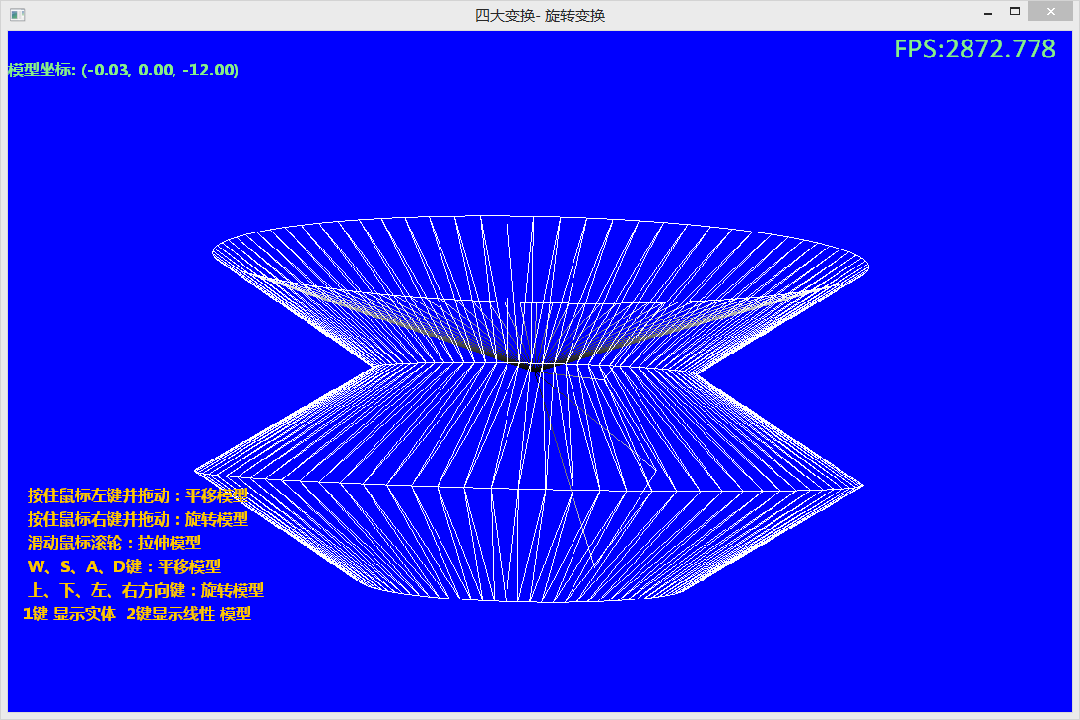
\includegraphics[angle=0,width=8cm,height=5.6cm]{DirectX-Rotation.png}%就在前面括号中写图片名
	 					\caption{Test图}
	 					\label{fig:winClass}
	 				\end{minipage}%
	 				\begin{minipage}[H]{0.5\textwidth} 
	 					\centering
	 					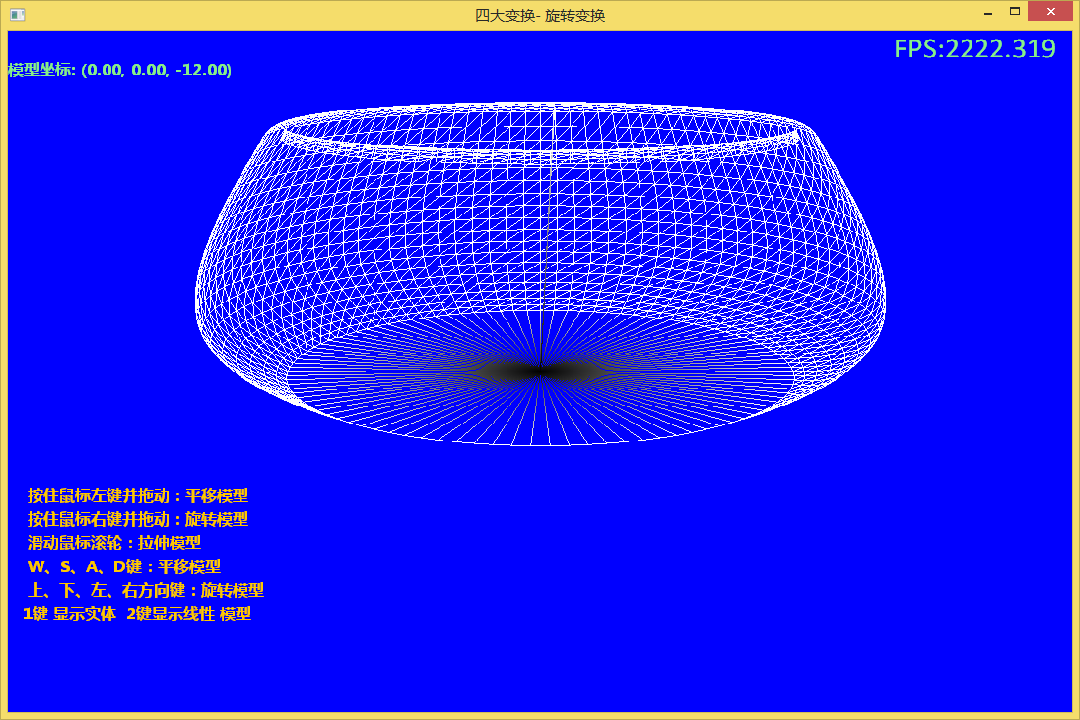
\includegraphics[angle=0,width=8cm,height=5.6cm]{Vase.png}
	 					\caption{Vase图 }
	 					\label{fig:createWindow}
	 				\end{minipage}
	 			\end{center}
	 		\end{figure} 	
		 	 
 	 \paragraph{Day 8       \quad     }
 	 \paragraph{Day 9       \quad     }
 	 \paragraph{Day 10      \quad     }
 	 \paragraph{Day 11      \quad     }
	 	 Hello  5.11:
	 	 
	 	 早上起床看了雷霆对阵马刺的天王山比赛的第四节, 雷霆获胜,听了会儿歌,
	 	 
	 	 给魏拓打了电话,问其是否已经上车或回家.问其何时归,
	 	 
	 	 与好久没联系的舍友章凌杰聊了会儿,同学的关系是不是就应该时不时的关心下,也许对于你来说是个可有可无的动作,但是对于授予者来说,可能会改变小伙的心态...
	 	 
	 	 
 	 \paragraph{Day 12      \quad     }
 	 \paragraph{Day 13      \quad     }
 	 \paragraph{Day 14      \quad     }
 	 \paragraph{Day 15      \quad     }
 	 \paragraph{Day 16      \quad     }
 	 \paragraph{Day 17      \quad     }
 	 \paragraph{Day 18      \quad     }
 	 \paragraph{Day 19      \quad     }
 	 \paragraph{Day 20      \quad     }
 	 \paragraph{Day 21      \quad     }
 	 \paragraph{Day 22      \quad     }
 	 \paragraph{Day 23      \quad     }
 	 \paragraph{Day 24      \quad     }
 	 \paragraph{Day 25      \quad     }
 	 \paragraph{Day 26      \quad     }
 	 \paragraph{Day 27  最近喜欢上了一个妹子    \quad     }
	 	 hello 5.27:
	 	 
	 	 今天星期5,这件事情发生在星期2上英语外教课时,对后面的妹子有好几次的冲动,就是张不开嘴,喜欢化成了懦弱,真正的喜欢可能就是这样,然后她说话了...她好像懂似的,然后我开始从上自然辩证法开始回忆,你好像是老坐在那个角落(阶梯)的女生,上课自拍的照片刚好被我抓拍到了...
	 	 
	 	 你是学硕?她开口问我..
	 	 
	 	 嗯,你也是学硕吧..那留个电话..再加个微信吧..
	 	 
	 	 回来兴奋的不知如何是好..下午吃完饭在操场上打球,心里满满的都是她..
	 	 
	 	 回来不知怎么开口跟她聊天..然后就翻看着她的状态..
	 	 
	 	 my God! 篮球妹子,吉他妹子, 西餐妹子, 自拍妹子....太多的相同点,然后因为最近也在练吉他,然后就找到那条状态评论了下...
	 	 
	 	 话题开始了...
	 	 
	 	 没想到..如此竟然结识了可能是性格最像的一个人了吧..真希望能让她做我女朋友,追她的人太多,我害怕给不了她要的幸福... 
	 	 
	 	 第二天...不想主动的联系...但是我真的好向往你..看着你推荐的小说《从你的全世界路过》
	 	 
	 	 第三天...打完球...猪头520..跟你聊天就是很开心...
	 	 
	 	 前段时间考到一本书,然后-“我希望成为那个对的时间遇到对的人的人”,那时我懂的如何爱,你懂的我爱你..要是再好点,成为彼此的另一半...
	 	 
	 	 最近,我喜欢上一个妹子...她叫陈瑞,她是我的红酒..
	 
 	 \paragraph{Day 28      \quad     }
 	 \paragraph{Day 29  美少女...换头像  \quad     }
 	 HELLO 2016.5.29:
 	 
	 	 感觉好幸福, 因为说了她头像笑的不是很开心,然后就换了好几次... 
	 	 
	 	 谢谢你,陈瑞... 
	 	 
	 	 "喂, 是否可以再多一点"
	 	 
	 	 "再多一点"
	 	 
	 	 "听我说"
	 	 
	 	 "喂, 是否可以再多一点"
	 	 
	 	 "再多一点"
	 	 
	 	 "包容我的任性"
	 	 
	 	 "在拥有的瞬间"
	 	 
	 	 "似乎就要消失"
	 	 
	 	 "说给我听好吗"  
	 	 
	 	 "我爱你"
	 	 
	 	 "我爱你"
	 	 
	 	 "直到世界尽头"
	 	 
	 	 "笑着说"
	 	 
	 	 "你笨"
	 	 
	 	 "试着说出来"
	 	 
	 	 "我爱你" 
	 	 
	 	 "这件事"
	 	 
	 	 "并不简单"
	 	 
	 	 "希望可以懂得如何去爱"
	 	 
	 	 "我向天空许愿"
	 	 
	 	 "喂, 就算想要去了解"
	 	 
	 	 "也尽是些"
	 	 
	 	 "不明白的事情" 
	 	 
	 	 "所以我们无法"
	 	 
	 	 "融为一体"
	 	 
	 	 "两个人用尽全力拥抱"
	 	 
	 	 "有你在身边, 只是这样"
	 	 
	 	 "我的世界就"
	 	 
	 	 "焕然一新"
	 	 
	 	 "单调的景色" 
	 	 
	 	 "也映射出色彩"
	 	 
	 	 "重新握起不知不觉"
	 	 
	 	 "分开的手" 
	 	 
	 	 "一起走"
	 	 
	 	 "我懂的爱了吗"
	 	 
	 	 "轻轻的问那片天空"
	 	 
	 	 "即使终要分离"
	 	 
	 	 "的日子到来"
	 	 
	 	 "能够一天天"
	 	 
	 	 "思念着你"
	 	 
	 	 "就足够了" 
	 	 
	 	 "有一天懂的"
	 	 
	 	 "分离意义的日子会来临"
	 	 
	 	 "让我们立下誓言, 走向明天"
	 	 
	 		 	 "我爱你"
	 		 	 
	 		 	 "我爱你"
	 		 	 
	 		 	 "直到世界尽头"
	 		 	 
	 		 	 "笑着说"
	 		 	 
	 		 	 "你笨"
	 		 	 
	 		 	 "试着说出来"
	 		 	 
	 		 	 "我爱你" 
	 		 	 
	 		 	 "这件事"
	 		 	 
	 		 	 "并不简单"
	 		 	 
	 		 	 "希望可以懂得如何去爱"
	 		 	 
	 		 	 "我向天空许愿"	 	
	 		 	 
	 		 	 
	 	心灵阅历:不要急于批判眼前看到的事物,因为那不一定就是你认为的真相.. 	 	 	 	 	 	 	 
	 
	 	心灵阅历:重要的不是什么都拥有, 而是你想要的恰好在身边...	 
 	 \paragraph{Day 30   最远的距离-泰戈尔   \quad     }
	 	 Hello 5.30:
	 	 
	 	 晚上看了《围城》:唐晓芙,一个秀外慧中的精灵般的女孩。在方鸿渐心中,那就是一块完美无暇透着宝气的美玉。 
	 	 
	 	 苏文纨,表面端庄,却傻得彻底且自私的半老徐娘。聪明的女孩是不会读那华而不实的博士的。 
	 	 
	 	 方鸿渐,懦弱却俏皮,简单又真实的男人。 
	 	 
	 	 方鸿渐拒绝了苏文纨,苏却在唐晓芙面前挑拨了唐和方,感觉受到欺骗的晓芙和鸿渐那面对面的爱与恨、倔强与懦弱之斗争让人揪心不已: 
	 	 
	 	 唐:我爱的人,我要占有他的整个生命,他在碰到我之前,没有过去,留着空白等着我……方先生,我只希望你前途无量! 
	 	 
	 	 方:是我不好……我是个骗子……我以后,也绝不来讨厌了。 
	 	 
	 	 唐:……鸿渐……远行……一路平安…… 
	 	 
	 	 方:…… 
	 	 
	 	 唐是表面倔强内心脆弱,方是懦弱却无奈。两颗相爱的心在面子面前是如此不堪一击,让人不禁想起了泰戈尔的那首
	 	 
	 	 \subparagraph{“最远的距离”}泰戈尔
	 	 
	 	 世界最远的距离 
	 	 
	 	 不是 生与死 
	 	  
	 	 而是 我站在你面前你却不知道我爱你 
	 	 
	 	 世界最远的距离 
	 	 
	 	 不是 我站在你面前你却不知道我爱你 
	 	 
	 	 而是 明知道彼此相爱却不能在一起 
	 	 
	 	 世界最远的距离 
	 	 
	 	 不是 明知道彼此相爱却不能在一起 
	 	 
	 	 而是 明明无法抵抗这股思念 


	 	 却还故意装作丝毫不把你放在心里 
	 	 
	 	 世界最远的距离 
	 	 
	 	 不是 明明无法抵抗这股思念  
	 	 
	 	 却还故意装作丝毫把把你放在心里 
	 	 
	 	 而是 用自己冷漠的心 对爱你的人 
	 	 
	 	 掘了一条无法跨却的深渠 
	 	 
	 	 \subparagraph{感悟}
	 	 懦弱使鸿渐失去了晓芙,鸿渐却也明白了——爱情、婚姻、职业……人生的欲望大抵都是一座围城,城里的人想逃出来,城外的人想冲进去。用他自己的话说,爱情就像狗咬着的骨头在水里的影子,人追求的是骨头的影子,是一个美丽的乌托邦,如果真要是吃了那现实中的骨头就会感到味道不过如此,所以最美的还是那影子。理性的分析的确如此,没得到时可以这样聊以自慰。然而,作为理性与感性交融的人,谁又逃脱得了感情的魔咒!鸿渐永远都超脱不了晓芙!所以,当赵辛楣戏谑鸿渐提到晓芙时,鸿渐会生气、会动怒走开……是啊,虽然经历后,我们会心静如水,但那个曾经在我们心中留下深刻印记的人,就像一块抛入湖面的小石子,会溅起阵阵涟漪……
 	 \paragraph{Day 31      \quad     }
 \section*{June}
 	 \paragraph{Day 1       \quad     }
 	 \paragraph{Day 2   Hello 6月    \quad     }
	 	 Hello 连续3天的雨天,失去了前进的方向,看着书也没感觉...
 	 \paragraph{Day 3  总决赛第一天,骑士输了但     \quad     }
	 	 Hello 
	 	 
	 	 早上被心爱的陈瑞叫醒,就算是昨天晚上安顿的..至少她把我记在心里了
	 	 
	 	 然后上了课,早起真的很不错
	 	 
	 	 下午打球了,发现自己对篮球的感觉越来越好...突破变得犀利,投篮变得精准
	 	 
	 	 晚上则洗衣服..
	 	 
	 	 
 	 \paragraph{Day 4       \quad     }
 	 \paragraph{Day 5   文泉与胖子来了   \quad     }
	 	 Hello :
	 	 
	 	 先说说感情的事吧,她这两天比较忙,感觉也淡了...老是忙,这感觉好像对自己不感兴趣的妹子一般
	 	 
	 	 下午文泉与胖子说要来,见了好久没见的挚友...聊了社会,聊了自己的见识,聊了格局,聊了发型...
	 	 
	 	 可是我的情绪现在比较低落...
 	 \paragraph{Day 6       \quad     }
 	 \paragraph{Day 7   发现真相的我眼泪掉下来... \quad     }
	 	 Hello :
	 	 
	 	 早上期待的上课,下午则在上课聊了好久..
	 	 
	 	 是不是宁愿不要问杨凌有什么好吃的.. 然后下午就不回去了..
	 	 
	 	 我宁愿被蒙到鼓里..
	 	 
	 	 下午吃凉皮的时候李嵩告诉我了她前段时间看到的东西,,回来的时候又看到了... 是不是6月7日是我的生命决定日..
	 	 
	 	 庆幸自己还没有开始恋爱..
	 	 
	 	 就不能好好的相处吗?
	 	 
	 	 我认识了一个妹子,她叫陈瑞..然后就知道了她挺会撒谎的... 其实我还是挺喜欢她的..
	 	 
 	 \paragraph{Day 8       \quad     }
 	 \paragraph{Day 9       \quad     }
 	 \paragraph{Day 10      \quad     }
 	 \paragraph{Day 11      \quad     }
 	 \paragraph{Day 12      \quad     }
 	 \paragraph{Day 13  好几天了..    \quad     }
	 	 Hello 你好:
	 	 
	 	 《守旧》
	 	 
	 	 你是深山的游客
	 	 
	 	 边走边爱四海为家 \hspace{1cm} 生性多情
	 	 
	 	 我是集市里的养猫者 
	 	 
	 	 不看路人  \hspace{1cm}  不换爱人
	 	 
	 	 你这话说给谁听,如果知道你有男友,我可能连你都不会认识...这就是我,简单的我
	 	 
	 	 自从那日她说谎后,我对她的印象便一落千丈,这就是我,简单的我
	 	 
	 	 如果没有奢望,便不会有失望
	 	 
	 	 那日如果能将你搂在怀里,,也许不会失去那段值得回忆的美好..
	 	 
	 	 不过你给了我一段美好的回忆,我还曾经甚至 不断幻想着咱俩结婚生子,,
	 	 
	 	 天真的金牛,
	 	 
	 	 太傻,太笨...给我一个女生,也许现在就可以陪她走到最后..
	 	 
	 	 我喜欢你是认真的..但是这就是命..你的话也是我的话.  再见!或许再 也 不 见
 	 \paragraph{Day 14      \quad     }
 	 \paragraph{Day 15      \quad     }
 	 \paragraph{Day 16      \quad     }
 	 \paragraph{Day 17      \quad     }
 	 \paragraph{Day 18      \quad     }
 	 \paragraph{Day 19      \quad     }
 	 \paragraph{Day 20  骑士赢了-见证詹姆斯逆转    \quad     }
	 	 相信一切皆有可能
	 	 
	 	 
	 	 他对家乡的报答, 他的落叶归根,他的落泪夺冠..
	 	 
	 	 你懂多少,你能做多少
	 	 
	 	 他对朋友的慷慨,对社会的奉献,对子女的教育
	 	 
	 	 你懂多少,你能做多少
	 	 
	 	 他是你的道德榜样,他是你的篮球教父..
	 	 
	 	 你理解的慢可以,但是你应该理解
	 	   
	 	 http://www.pudaquan.com/html/jitapu/10\_870\_1.html
 	 \paragraph{Day 21      \quad     }
 	 \paragraph{Day 22      \quad     }
 	 \paragraph{Day 23   美少女   \quad     }:
 	    正着念和反着念完全不同
 	    
	 	 WE are a part of Generation that has never seen a Cleveland Championship.
	 	 
	 	 I  Realize this may be a Shock BUT
	 	 
	 	 We Can  Help OUR Team win a title
	 	 
	 	 Is A lie, AND
	 	 
	 	 We are  the mistake  by the lake
	 	 
	 	 so in 30 years i will tell my children
	 	 
	 	 How Close We Were,
	 	 
	 	 The shot, The Drive, And the 9Th inning collapse.
	 	 
	 	 We can forget about 
	 	 
	 	 winning the big ONE
	 	 
	 	 Nothing happens here except
	 	 
	 	 APATHY and SELF-PITY
	 	 
	 	 WE CAN  dispose of
	 	 
	 	 Dreams
	 	 
	 	 Reality  overtakes the
	 	 
	 	 MISSION
	 	 
	 	 WE cannot be deterred from the
	 	 
	 	 Image of a Buring River
	 	 
	 	 WE no longer emboody the 
	 	 
	 	 Championship Image
	 	 
	 	 United we show a 
	 	 
	 	 collective failure
	 	 
	 	 We Do not believe in
	 	 
	 	 ONE GOAL...
	 	 
	 	 And 
	 	 
	 	 all of this will come true
	 	 
	 	 unless we choose to
	 	 
	 	 REVERSE IT...
 	 \paragraph{Day 24      \quad     }
 	 \paragraph{Day 25      \quad     }
 	 \paragraph{Day 26      \quad     }
 	 \paragraph{Day 27      \quad     }
 	 \paragraph{Day 28      \quad     }
 	 \paragraph{Day 29      \quad     }   
 	 \paragraph{Day 30      \quad     }
 	 \paragraph{Day 31      \quad     }
 \section*{July}
 	 \paragraph{Day 1   晚上的聊天感觉挺有用    \quad     }
	 	 Hello 7月:
	 	 
	 	 都不知道世界怎么能过的如此之快..因为自己学的东西少了,因为过程太过单调单一..
	 	 
	 	 当你失去前进的目标时,找找你当时渴望得到的东西得到了吗...
	 	 
	 	 "你要知道陷在消极里没有用,只有行动才能改变焦虑,担心什么就去做什么"-陈瑞说了一句我原来一直想知道而不知道的道理,谢谢你,虽然可能不能陪我走完这辈子,但是你的出现真的很开心..
	 	 
	 	 "当你明白变优秀比什么都重要的时候,就再也没时间干其他无用的了.."
	 	 
	 	 开始记录你的日子吧,要不时间和过程都不知道怎么过去的..	 
 	 \paragraph{Day 2       \quad     }
 	 \paragraph{Day 3       \quad     }
 	 \paragraph{Day 4       \quad     }
 	 \paragraph{Day 5   这样的日子    \quad     }
	 	 Hello 7.5:
	 	 
	 	 还记得去年搬下去下的决心,可是今天却知道人心冷暖a..
	 	 
	 	 就这样被美丽老师放弃了吗? 范玉玲啊... 社会的事还是你懂的比较多..
	 	 
	 	 加油,现在经历的都是给以后铺路..别哭
	 	 
	 	 乖,摸摸头..
 	 \paragraph{Day 6       \quad     }
 	 \paragraph{Day 7       \quad     }
 	 \paragraph{Day 8       \quad     }
 	 \paragraph{Day 9       \quad     }
 	 \paragraph{Day 10      \quad     }
 	 \paragraph{Day 11      \quad     }
 	 \paragraph{Day 12      \quad     }
 	 \paragraph{Day 13  旅行的意义    \quad   小雨,微凉  }
	 	 Hello 7.13:
	 	 
	 	 读万卷书,行万里路,这个古人告诉我们的旅行的意义。即所谓阅历。
	 	 
	 	 行走,不停歇的行走,意义就在脚下,有人其实就是在边旅行边探寻人生的意义。
	 	 
	 	 只有一个人在旅行时,才听得到自己的声音。它会告诉你,这世界比想象中的宽阔。你的人生不会没有出口,你会发现自己有一双翅膀,不必经过任何人同意就能飞!
	 	 
	 	 我们常常看到的风景是:一个人总是仰望和羡慕着别人的幸福,一回头,却发现自己正被仰望和羡慕着。其实,每个人都是幸福的。只是,你的幸福,常常在别人眼里。
	 	 
	 	 你是一树一树的花开,是燕在梁间的呢喃,你是爱,是暖,是希望,你是人间的四月天。”(林徽因)又是一年的四月,春暖花开,桃红柳绿,莺啼燕语,正是最适合出游的时节。
	 	 
	 	 想起钱钟书的一句话:“要想结为夫妻,先去旅行一次”,给单身的大家出个馊主意:如果,对一个人,是取是舍,很矛盾要不要选择他的时候,就和他出去旅行吧。通过他的待人接物,处理问题,照顾他人……检验他的耐心度,细心度,处理问题的能力……
	 	 
	 	 美景不仅仅是目的地,还应该是在路上,旅行也不仅仅是目的地,还在感受沿途的那些人那些事,那些曾经发生在这片土地上的点点滴滴。
	 	 
	 	 旅行之意义并不是告诉别人“这里我来过”。是一种改变。旅行会改变人的气质,让人的目光变得更加长远。在旅途中,你会看到不同的人有不同的习惯,你才能了解到,并不是每个人都按照你的方式在生活。这样,人的心胸才会变得更宽广,我们才会以更好的心态去面对自己的生活。
	 	 
	 	 
	 	 \textbf{日子过得迷茫也得前行,因为回首往事时,你会感激自己曾经积累的硅步}
	 	 
	 	 不积硅步,无以至千里,这是我研究生学到最重要的一个道理
 	 \paragraph{Day 14      \quad     }
 	 \paragraph{Day 15      \quad     }
 	 \paragraph{Day 16      \quad     }
 	 \paragraph{Day 17      \quad     }
 	 \paragraph{Day 18  迷失又出现在笔记里    \quad     }
	 	 Hello:
	 	 
	 	 不知道咋地,疯了般的玩了3天的游戏..,原计划的好好学习,好好的读论文,却现在变成如此...
	 	 
	 	 仅反思。
 	 \paragraph{Day 19      \quad     }
 	 \paragraph{Day 20      \quad     }
 	 \paragraph{Day 21  有些事终于发生了    \quad     }
	 	 Hello 21:
	 	 
	 	 早上打热水的时候,突然收到信息说下午要开组会,激动但又异常的奇怪..
	 	 
	 	 开会的时候,洋哥汇报了他的成果,虽然没有作多少,却让听的人感觉好多...这就李老板口中的好样子
	 	 
	 	 陈志涛的汇报,确实感觉人家学到了好多,也就1年的时间,他真的学到了好多,JavaEE,Jquery,Hadoop 等,而且口才也因为干了事而脱口而出...
	 	 
	 	 接下来的我们,不评论了..
	 	 
	 	 后来,李老板突然指出,美丽老师说郑华你不好带,当时虽然晴天霹雳,但是我已经意识到了这一点,因为一学期都没找美丽姐了,所以啊,正常
	 	 
	 	 没项目,没人带.... 啊,快疯了,我想哭
	 	 
	 	 还好,看到王迪小子分享的一段文字“生活在地球上,与天地同在,与万物同生,有意思”,生活本来就要学会独立..加油
 	 \paragraph{Day 22      \quad     }
 	 \paragraph{Day 23  写了致歉信    \quad     }
	 	 hello:
	 	 
	 	 致歉信如下:
	 	 
	 	 尊敬的美丽老师:
	 	 
	 	 想了好几天,但是还是没有勇气打通你的电话,心中有些东西还是不知道怎么陈述。
	 	 
	 	 起初,从403搬下来,本应该先与美丽姐您打招呼的,可是当时真的比较情绪化,回过头来想起,这一切的后果我必须承担。
	 	 
	 	 后来,从303搬回宿舍,没有想太多,因为宿舍刚装修,环境不错而且比较清静,又有几个关系比较好的也搬回了宿舍,没有意识到导师们其实挺看重你是否积极的到实验室这个问题。
	 	 
	 	 关于项目,美丽姐可能考虑的太多,老是问我喜欢做什么,然后这个问题我就认真的回答了,当我回答了自己比较向往做游戏时,只是在陈述而已,并没有暗示我只 做与我相关的,我可以区别什么是喜欢什么是工作或学业,你可以直接安排-需要我作的,可以帮你做的,必须做的。而且我会,也愿意努力完成它。 我觉的咱们最大的误会可能就在这了。
	 	 
	 	 美丽姐,当徐杨老师说要走时,我真的很担心自己,可是听到是美丽老师会指导我,真的是吃了定心丸。
	 	 
	 	 美丽姐,如果我做错了,请指责我,我真的不是刻意要造成这些的。
	 	 
	 	 美丽姐,对不起。
	 	 
	 	 第二天早上收到了美丽老师的回复,真的万幸,并且越了7.25 下午见面谈。
 	 \paragraph{Day 24      \quad     }
 	 \paragraph{Day 25   见了美丽老师,其实并没有那么差   \quad     }
	 	 Hello,
	 	 
	 	 早上看了比赛,中国队输的比较惨,主要还是因为紧张吧
	 	 
	 	 下午美丽姐发来消息说帮取快递,然后在超市等她,聊了一路,感觉其实挺好,然后确定了要编写的代码
	 	 
	 	 \textbf{确定每周至少一次汇报,通过Emil}
	 	 
	 	 加油,可以的
 	 \paragraph{Day 26   调试代码   \quad     }
	 	 Hello:
	 	 
	 	 感觉今天其实挺充实的..
 	 \paragraph{Day 27      \quad     }
 	 \paragraph{Day 28   大神的代码与业余的区别   \quad     }
	 	 Hello:
	 	 
	 	 睡觉前,因为变换着急的睡不着,结果一下就找到了一个惊人之作,大神作品映射,与投影,并截图对比
		 
		 \begin{figure}
		 	\begin{center}
		 		\begin{minipage}[H]{0.5\textwidth}
		 			\centering
		 			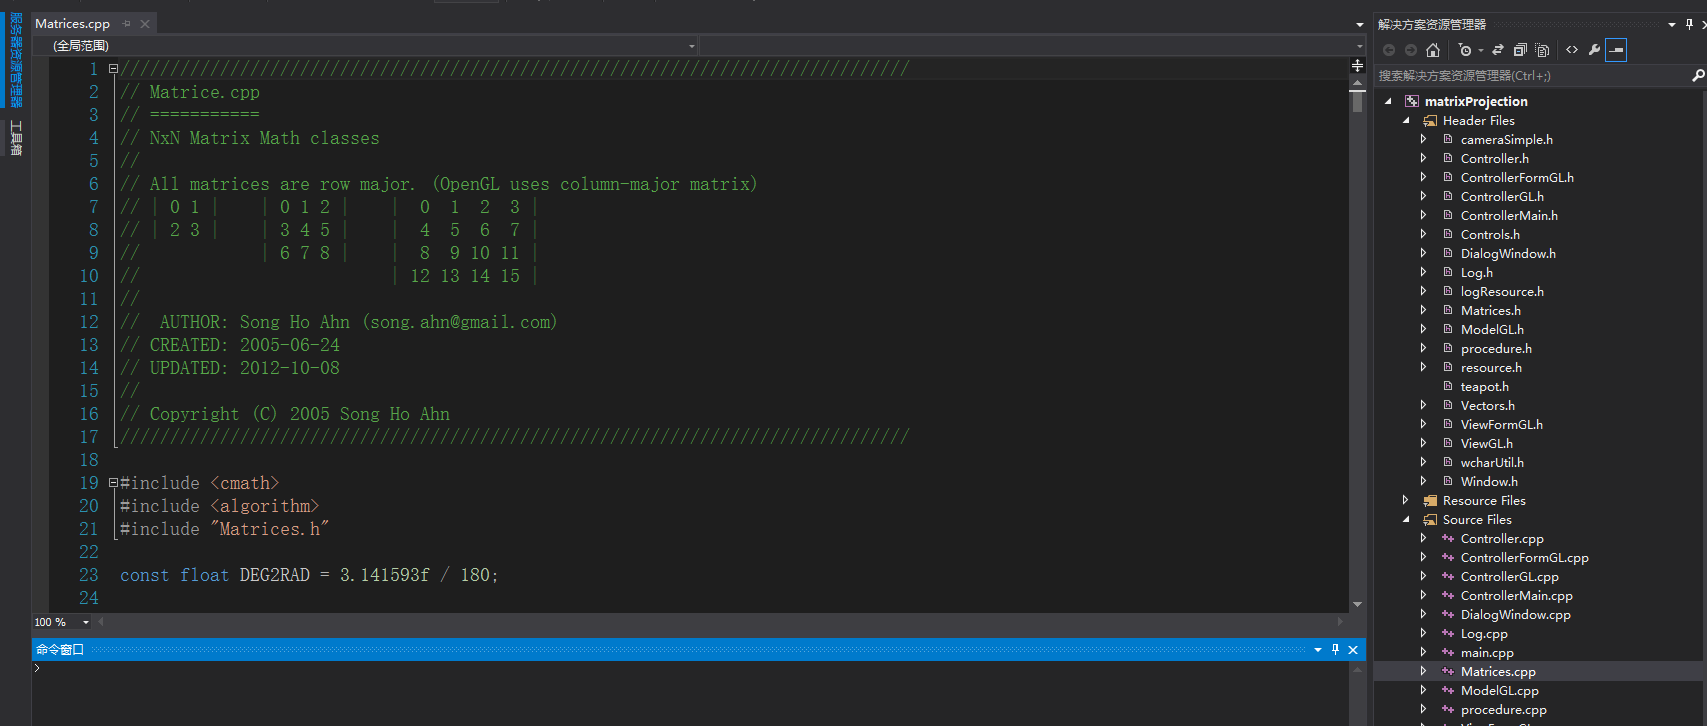
\includegraphics[angle=0,width=8cm,height=5.6cm]{good.png}%就在前面括号中写图片名
		 			\caption{大神图}
		 			\label{fig:Good}
		 		\end{minipage}%
		 		\begin{minipage}[H]{0.5\textwidth} 
		 			\centering
		 			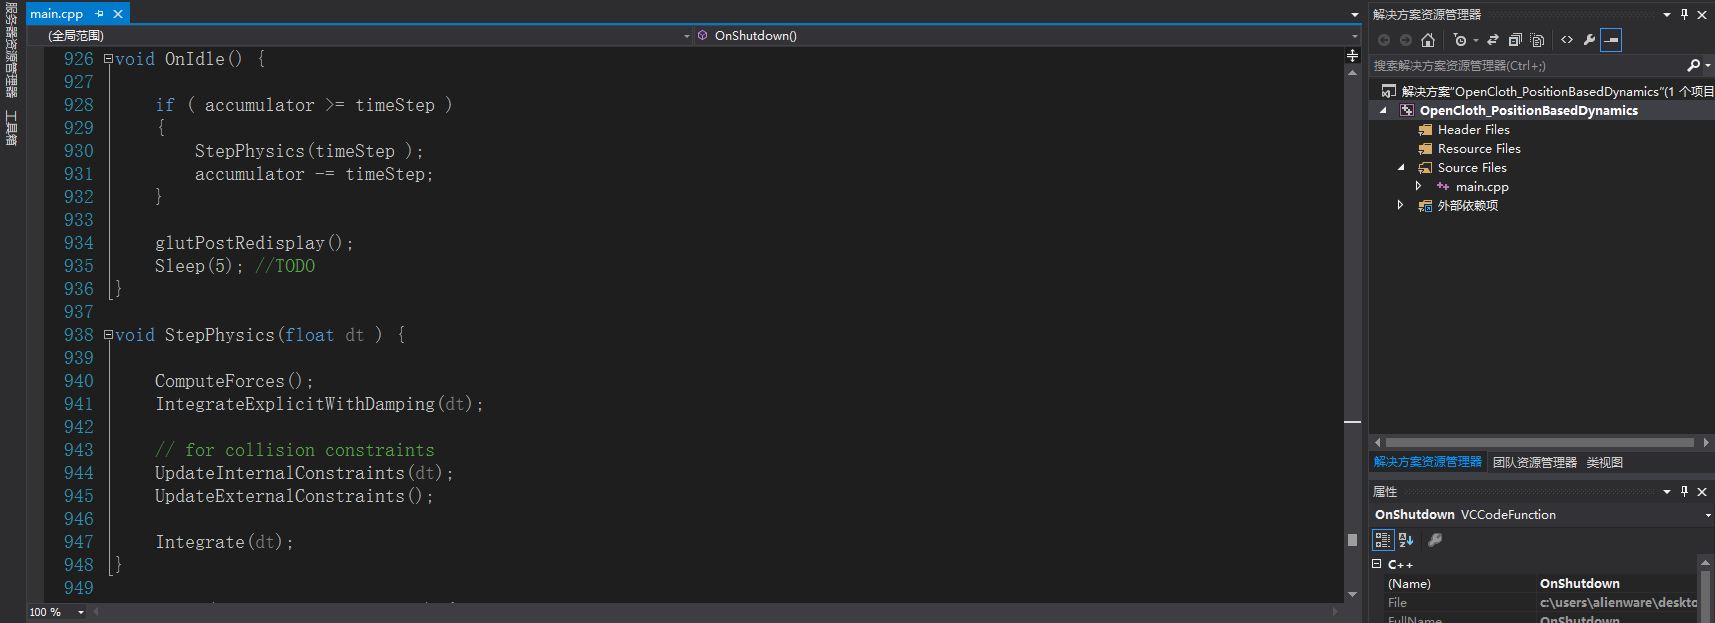
\includegraphics[angle=0,width=8cm,height=5.6cm]{bad.png}
		 			\caption{业余图 }
		 			\label{fig:Bad}
		 		\end{minipage}
		 	\end{center}
		 \end{figure} 
		 
		 \begin{figure}
		 	\begin{center}
		 		\begin{minipage}[H]{0.5\textwidth}
		 			\centering
		 			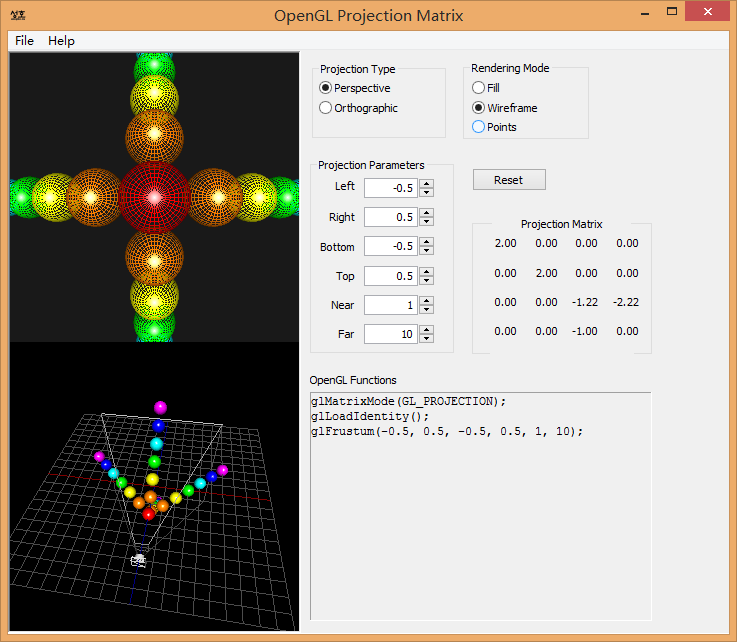
\includegraphics[angle=0,width=8cm,height=5.6cm]{good2.png}%就在前面括号中写图片名
		 			\caption{大神图}
		 			\label{fig:Good2}
		 		\end{minipage}%
		 		\begin{minipage}[H]{0.5\textwidth} 
		 			\centering
		 			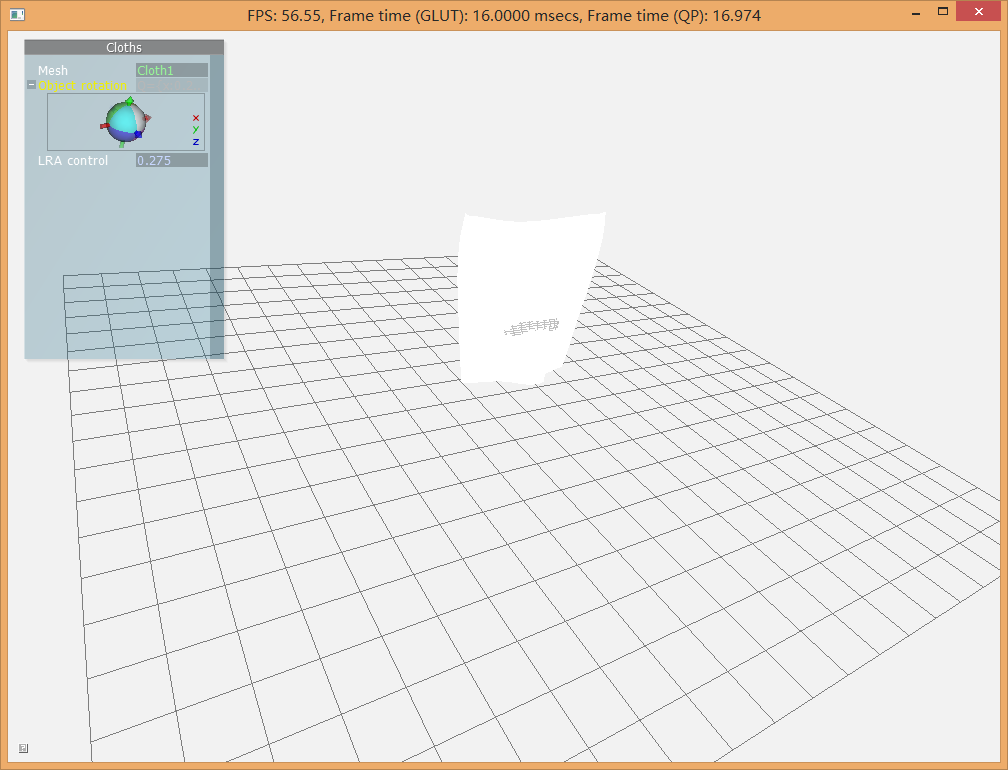
\includegraphics[angle=0,width=8cm,height=5.6cm]{bad2.png}
		 			\caption{业余图 }
		 			\label{fig:Bad2}
		 		\end{minipage}
		 	\end{center}
		 \end{figure}		 
 	 \paragraph{Day 29      \quad     }   
 	 \paragraph{Day 30  汇报并受到表扬    \quad     }Hello:
 	 
	 	 表扬的力量是无穷的,但是实在的干事是最主要的
	 	 
	 	 这几天的日程见2016年网易邮箱:“2016-7.26至今事宜”
 	 \paragraph{Day 31      \quad     }
 \section*{August}
 	 \paragraph{Day 1       \quad     }
 	 \paragraph{Day 2       \quad     }
 	 \paragraph{Day 3       \quad     }
 	 \paragraph{Day 4       \quad     }
 	 \paragraph{Day 5  跟老爸通了电话,感觉他心情并不是很好   \quad     }
	 	 Hello:
	 	 
	 	 发现,学习这方面看论文,真的挺快的,尤其是概述,感觉瞬间就可以对一个学科有一定的了解。
	 	 
	 	 知道了一些杂志排名:http://www.ccf.org.cn/sites/ccf/biaodan.jsp?contentId=2903940690854
	 	 
	 	 关于投论文:http://muchong.com/html/201408/7774210.html
	 	 
		 见根目录《计算机图形学与多媒体》
 	 \paragraph{Day 6       \quad     }
 	 \paragraph{Day 7       \quad     }
 	 \paragraph{Day 8   跟了英国国家动画中心的乾坤师兄确定了方向    \quad     }Hello:
 	 
	 	 下午打了球,然后做了瑜伽,哦,晓东今天回来了。
	 	 
	 	 晚上回来跟钱坤师兄确定了 要研究的方向(加速收敛)。
	 	 
	 	 感觉对 陈瑞没感觉了,主要是因为 她的那几次骗人。
 	 \paragraph{Day 9       \quad     }
 	 \paragraph{Day 10  看文章发现问题    \quad     }
	 	 Hello :
	 	 
	 	 看文章发现 有一个程序中的参数一直不明白是什么意思,$w_i$,先是美丽姐估计是 权重,后钱坤大师讲解了下,看来理解的差不多,唯一的不懂就是在 那个均化 变化值的地方没弄明白。
	 	 
	 	 加了钱大师的微信,发现留学英国真的很不错。见识确实会得到很大的提升。
	 	 
 	 \paragraph{Day 11      \quad     }
 	 \paragraph{Day 12      \quad     }
 	 \paragraph{Day 13      \quad     }
 	 \paragraph{Day 14      \quad     }
 	 \paragraph{Day 15      \quad     }
 	 \paragraph{Day 16      \quad     }
 	 \paragraph{Day 17   算是把段茹香当成朋友了吧   \quad     }Hello:
 	 
 	 对这两天看的论文整理了问题,向钱师兄请教了下。非常感谢钱师兄如此慷慨的为我解决问题,如果是自己早都不耐烦帮我解决这个问题了。
 	 
 	 发现在对文章的理解,还有兴趣这方面等跟段茹香还是挺像的,主要他对我感觉说话没有隐藏(什么手印之类了),所以还是能交就把握。
 	 
 	 知道了吉他的面单和全单的区别。
 	 
 	 \paragraph{Day 18      \quad     }
 	 \paragraph{Day 19      \quad     }
 	 \paragraph{Day 20   又是钱郑大论   \quad     }
	 	 Hello:
	 	 
	 	 晚上热的睡不着,跑起来写代码,但是对几个点没有理解到位还是不得不停下来。
	 	 
	 	 中午,坤哥与我又上演了坤郑各不服 的争论场面。
	 	 
	 	 不过还好,有些东西真的是没理解到位,也没注意,\textbf{所有现在看别人的评价感觉不对,可能完全是因为自己的层次还没到那种地步或者格局。}
	 	 
	 	 读论文一句句的读,别偷工减料,很关键,而且每一句都得弄明白。
	 	 
	 	 论文间的联系该怎么体现也是个学问。
	 	 
	 	 论文的书写与内容:漂亮很重要,内容反而并没有占多少。
	 	 
	 	 我愿意当苦力,只是因为我缺少实践,而且我也想报答这份老师对我的恩情。
	 	 
	 	 加油。
 	 \paragraph{Day 21      \quad     }
 	 \paragraph{Day 22      \quad     }
 	 \paragraph{Day 23   WT回学校了,打球被虐了   \quad     }Hello:
 	 
 	 欧文的那招确实是个奇招..
 	 
 	 打印了论文,准备复习下网络编程,不对,是学习。
 	 
 	 明天的boost 书就到 了,好兴奋。
 	 \paragraph{Day 24      \quad     }
 	 \paragraph{Day 25      \quad     }
 	 \paragraph{Day 26      \quad     }
 	 \paragraph{Day 27      \quad     }
 	 \paragraph{Day 28      \quad     }
 	 \paragraph{Day 29      \quad     }   
 	 \paragraph{Day 30      \quad     }
 	 \paragraph{Day 31      \quad     }
 \section*{September}
 	 \paragraph{Day 1       \quad     }
 	 \paragraph{Day 2       \quad     }
 	 \paragraph{Day 3  回忆下这段时间     \quad     }
	 	 Hello:
	 	 
	 	 前段时间,李嵩出去玩叫了很多人,然而,没有叫我。我以为是别人组织的...
	 	 
	 	 后来,魏拓告诉了我..
	 	 
	 	 最近,学院实验室要接新生,我要送文浩,因为这个是朋友,我选择了不去参加那个新生的聚餐.
	 	 
	 	 后来, 感觉李嵩还是与自己的朋友标准有些差距,
	 	 
	 	 让我想起了那句话“哪有人喜欢孤独啊,只是不希望失望罢了”
	 	 
	 	 昨天被老范叫出去说要让请吃饭..然后看着对面的两位女生,不知当时自己在想着什么,不禁问自己..我的另一半真的遇到就这么难么..
	 	 
	 	 生活的辛酸滋味、生活的甜蜜、当然这些都得体验,然而这种被欺骗的感觉真的受不了,这种失望的感觉真的不想再有.
	 	 
	 	 但是,没有辛酸,哪知道甜蜜就是甜蜜。
 	 \paragraph{Day 4   水街-茯茶-乐华 之旅    \quad     }Hello:
 	 
	 	 早上起来,与晓东在门口吃了潼关肉夹馍,然后开始我们的旅行.
	 	 
	 	 魏拓开着车,有点担心,老实说..
	 	 
	 	 不一会\textbf{水街到了},只能说相对的话,规模还是有点小。但是里面还是最近发展的可以,只是不再只有买麻花的.吃了个比脸还大的鸡排,味道真的不错。然后转着,景区的东西确实贵..10元每个冰棍,当然最美的还是水旁边的街道,与水上的道路
	 	 
	 	 下午决定先到茯茶小镇吃个小吃填填肚子,然后导航的延时导致错过出口,中间耽搁了些时间.
	 	 
	 	 \textbf{到达茯茶小镇后},各种商品映入眼帘,首先是“茯茶”,我只想说,就算是活菌,也经不住高温。其次就进入了小吃街,喝了茯茶奶-甜中带苦,去除了其油腻的感觉,再加上冰镇的效果-不错。 然后是 菜卷,凉粉、搅团,味道还不错,只是确实小贵。接着的是鸭血粉丝汤,只鞥说15元买的东西只能填饱肚子,味道与马嵬驿的还是有些差距。 然后存宝吃了夹馍过来,请了我们吃了烤串,然后这个烤串的出现确实让人意向不到,这促使了他生意的火爆。最后,哪都有凉皮。
	 	 
	 	 回车上的时候,路过书法的地方,很美,但实在没有能力帮他们一把。
	 	 
	 	 \textbf{欢乐谷到了}。
	 	 
	 	 1- 飞艇是第一个,开始有些担心,最后发现并没有什么,不过挺爽的..
	 	 
	 	 2- 跳楼机是第二个,你敢信!我都佩服自己的勇气,但是停留在高空眺望远方的感觉真的是深深的刻入脑海,冲下的时候,喊出来的时候就像获得新生般,刺激但又有别的不一样的感觉,说不出来.(回头想起那个画面真的还挺后怕的)
	 	 
	 	 3- 冲水船吧,往下冲有点过山车的感觉,但是水花四溅的感觉冰凉的让人不敢睁开眼睛..还不错
	 	 
	 	 4- 空中摩托,激烈的加速,瞬间感觉就要被气流冲走,倒挂的瞬间,还有随着摩托的左右翻身,..很开心
	 	 
	 	 5- 流星锤是最后的也是感触最多的,到达顶峰感觉要往下掉的感觉,到达低处脚底充血的感觉,当然,还有高空中各种无意识的呐喊,身心和灵魂得到了释放
	 	 
	 	 回来的路上,又是导航的问题,折腾了很久。
	 	 
	 	 肚子难受,但心里开心,今天完成了这几年都没有完成的挑战。最重要的是意识到一点:“\textbf{摆在你面前的困难可能看起来十分恐怖,但是你不尝试,永远不知道其实它不值得一提!最重要的是,你要踏出尝试的步伐和实践的脚步}”
 	 \paragraph{Day 5       \quad     }
 	 \paragraph{Day 6       \quad     }
 	 \paragraph{Day 7       \quad     }
 	 \paragraph{Day 8       \quad     }
 	 \paragraph{Day 9       \quad     }
 	 \paragraph{Day 10      \quad     }
 	 \paragraph{Day 11      \quad     }
 	 \paragraph{Day 12      \quad     }
 	 \paragraph{Day 13      \quad     }
 	 \paragraph{Day 14      \quad     }
 	 \paragraph{Day 15  8月15中秋佳节    \quad     }
	 	 Hello:
	 	 
	 	 先写昨日吧,因为还是比较有些东西值得回忆..
	 	 
	 	 雷东的小孩出月,没去..没礼...,结婚也没去,..没礼..
	 	 
	 	 下午决定参加303 的聚会,不一样的学妹让我耳目一新..有黑龙江豪爽的妹子..有陕西本土自大的姑娘,还有黑龙江被调侃的师妹... 能遇到就是缘分,内蒙古的陈利德,还有那个褚耀..感觉还是比较会处事..
	 	 
	 	 \textbf{礼仪在哪都不是可有可无的,虽然当时你觉得可以省略,是的...交际,可能就是在一次次的过程中学习技巧,体悟别人身上自己的影子犯的错误..}
	 	 
	 	 今天,是中秋..
	 	 
	 	 说好今天看电影,所以特别开心,不是因为电影,而是一起看电影的人..不是喜欢她的样子,而是喜欢她的身材..还有她的见识与层次.. 她懂得比我多..所以虽然不是自己喜欢的脸,但是还是想发生些什么..但是一旦有这样的想法就很危险,我是一个很容易为女生吃醋的那种..小心眼,是吧..
	 	 
	 	 她叫 李婷婷..不管结果怎样,她出现在了我的生活中,过程也罢,至少曾经一起有段这样的经历.
	 	 
	 	 话题还是找出来的,但是这些还是缘于积累,所以,用希区柯克的话说-\textbf{“如果喜欢一个人,不要让她无聊”}的最后方法就是自己学习,积累..
	 	 
	 	 回来的路上,接到父亲的电话,首先,我也很开心,因为至少现在还没有像陈勇老师那样没有后路的境遇..但是我还是担心,因为肺就像没有出口的迷宫,一旦陷进去,就真的出不来,我感到他对这个检测结构的满意,但是我也隐约听到他放松了对身体健康的警惕..我不想当检测出来后才痛彻心扉的体悟人生..我爱我的家人,但是我只能这样了..因为现在的我还无力实践,因为我的价值观最深的一层就是“做”,其他的都是扯淡..
	 	 
	 	 \textbf{心确实没有放到家上},这个本属于一家团聚的日子,我是个例外..怪就怪吧,我已经培养的性格,改需要时间..
	 	 
	 	 爸,你的身体和妈的身体是家的一切,这是我坚持到今天的最深的动力..一定要好好的..
	 	 
	 	 回到宿舍,带着气愤,感慨父亲的那般性格..但是这就是父亲,他给我的我不想只是背影..不知道他经历了什么,所以对他的思想、感悟、做法不了解,\textbf{也许,当我知道了他经历的事情后,他做的可能是最好的选择了已经..}
	 	 
	 	 身边的几个哥们,因中秋,下山小聚..畅述..
 	 \paragraph{Day 16      \quad     }
 	 \paragraph{Day 17      \quad     }
 	 \paragraph{Day 18      \quad     }
 	 \paragraph{Day 19      \quad     }
 	 \paragraph{Day 20   西安-电子科大南校行   \quad     }Hello:
 	 
	 	 村里呆久了,见识真的会酸化..好多的理想,好多的未来都会化成泡影..
	 	 
	 	 \subparagraph{人情篇:}说好的一起陪澤撸去西安参加宣讲会的,到最后都一个个因为天气放弃了陪伴的脚步..\textbf{人情本不该这样,越是艰难越是需要,不是吗?}
	 	 
	 	 早上11点左右离开杨凌,在魏家凉皮买了特色套餐,第一次吃肥肉夹馍吧,不太想让澤撸耗费..
	 	 
	 	 高铁上,吃着特辣的凉皮,没水,相视而笑..
	 	 
	 	 坐上公交,with raining, 到了..
	 	 
	 	 \subparagraph{感悟篇:}穿梭在西电南校的 奔驰,奥迪历历在目,回想自己母校那罕见的老总..辛酸,谁知。
	 	 
	 	 千回路转,终于找到了D楼,那么亲切,第一场是锐捷的,只招研究生..还挺高兴,第二场是浪潮的,...擦身而过手持LV的女生,高冷还有那气质..职场可能就是这样..
	 	 
	 	 令人难忘的 本校生(西电)的独白,满满的回忆,拼搏的身影..与那幽默的陈述,是的,应该给个赞,这就是积累和锻炼造就的..
	 	 
	 	 回来到钟楼开始我们的吃货旅途,奇怪的牛排,还有独特的小火锅,不会再来了..
	 	 
	 	 回来差点又赶不上火车了..还好赶上l..
	 	 
	 	 路上讨论这我们对书的看法,当然还有他的经历,那个高中的女孩,还有对生活的认识“有好必定有坏”
	 	 
	 	 回校,与婷婷聊天,但是隐约感觉男朋友的存在..这就是我奇怪的基因-爱怀疑,如果能单纯的生活就好了,不用那么复杂的活着,这社会会不会也会变得不那么尔虞我诈..\textbf{如果真的喜欢,你就该无理由的信任一个人..这是前提,也是基础..}
	 	 
 	 \paragraph{Day 21      \quad     }
 	 \paragraph{Day 22  澤撸回来了,山下又是一顿..    \quad     }Hello:
 	 
	 	 昨天晚上,因为婷婷的冷漠,也可能是自己想多了..打球后好累,洗完澡叫着魏拓到山下去吃北京古铜涮锅..
	 	 
	 	 今天..
	 	 
	 	 澤撸好像面试的不是很顺利,肯能那个场景自己就是懂也会因为紧张忘了吧..
	 	 
	 	 看到小伙子憔悴的面孔,还是感觉有些担心自己..
	 	 
	 	 找工作的压力瞬间就到了自己身上..
	 	 
	 	 但是,我们最相同的就是单身问题了,哈哈,这点永远有着探索的前景..当然今天就让他真诚的戳出了自己的脆弱.."如果有个男生和她聊的很嗨,你受的了吗",突然间好像被他知道了自己那段不成功的恋情一般,羞愧又愤怒,\textbf{朋友的真诚他做到了},当然我也就开始了自己的回应。“是的,我会吃醋,而且一般会特别生气”“还有不会追那种有男票的女生..”
	 	 
	 	 邹浩上场:“结婚了吗?法律有规定吗?”
	 	 
	 	 “吃醋,一定要让她知道,否则这种生气没什么用,而且会转化为冷战,对彼此都不好.还有,告诉她后看她的反应,再确定是否放手或继续..俗话说,有一有二无再三再四。  \textbf{而所有的前提就是-“沟通”!}”
	 	 
	 	 \textbf{“行动了那么你有50\% 机会, 不呢只有 0\%!”}w拖上场了..
	 	 
	 	 
	 	 睡觉前,澤撸通过了浪潮的面试..小伙子高兴的...
 	 \paragraph{Day 23      \quad     }
 	 \paragraph{Day 24      \quad     }
 	 \paragraph{Day 25  人生第一次参加领取奖学金的仪式   \quad     }
	 	 Hello:
	 	 
	 	 早上在各种思绪的敲击下起床了,洗了头,叫了魏拓,下山参加“晨露奖学金”的颁奖仪式,起初带着各种担心,因为自己的发型真的太起眼了,后来随着仪式的进行,担心终于没了..
	 	 
	 	 程安东 老省长开始了仪式的祝词,很是感慨,"\textbf{磨难是一份宝贵的财富}"。
	 	 
	 	 孙其信 校长的讲话也是真的很让人感悟,惟妙惟肖的停顿-引用程老的对话-古人的名言,让我知道了讲话的魅力..和诗书的境界。
	 	 
	 	 对这份奖学金的无比感激让我不禁想到父母的养育之恩的巨大..
	 	 
	 	 下午,开组会,锻炼自己口才.
	 	 
	 	 晚上,跟婷婷师妹聊天,好多经历,让我望尘莫及..虽然遥不可及,但是好想拥有..\textbf{这就是人,越是得不到越想得到..}
	 	 
	 	 晚上12:00 接婷婷回宿舍..有希望吗?
 	 \paragraph{Day 26      \quad     }
 	 \paragraph{Day 27   飞哥身体检测出双肾结石..魏拓23最后一天   \quad     }
	 	 Hello:
	 	 
	 	 今天是星期二,带着昨日剩下的早起余晖,起床看了会儿多线程..
	 	 
	 	 午饭吃了会儿..然后我就直白的告诉了魏拓当着人面算钱真的很伤人,感觉是伤着了彼此.脆弱的自尊心..
	 	 
	 	 爸妈在睡觉钱打来电话,说给打钱..觉得只有父母才会这样吧,无要求你回报得单纯付出..
	 	 
	 	 下午,午睡,先是听到飞哥接到老范的电话然后就去帮其搬桌子..然后迷迷糊糊的听到其焦急的声音和嘈杂的电话声-我以为是钱包丢了..没有上心..
	 	 
	 	 起床后,与澤撸一起吃了饭,为魏拓买了蛋糕..\textbf{有些事不是别人要求你做你再做,而是你必须做的,不管你要求否,做与不做是我的选择..是自己对自己的评鉴..}
	 	 
	 	 饭后回宿舍,飞哥疼痛难忍,陪着其到医院检测-就诊,最后各种医院的措施和最后的检测结果让彼此都不能自已.. “憋尿、B超、走路..当然还有段子..”
	 	 
	 	 送飞哥回宿舍后,准备魏拓的生日迎接仪式.
	 	 
	 	 与魏拓和澤撸一起取了蛋糕,到校门外买了吃的..啤酒、凉菜、鸡柳,当然还有调解气愤的烟..
	 	 当等到存宝出来后,\textbf{我们一起下山数台阶,,先下到最底层,然后往上数24层,庆祝WT的24岁生日..仪式随可有可无,但是这是我们纪念的途径,这是我们给他的Drama}
	 	 
	 	 面对对面的车海,面对逐渐远去的公路..当然还有即将随风而去的23岁..日子过着过着就又老了..
	 	 
	 	 \textbf{人如果矫情起来,感觉什么都是在写自己.."斜风细雨不须归!",还有绵绵秋风与你我共度}
	 	 
	 	 \textbf{我们彼此交流,彼此扯淡,彼此谈着自己内心的故事、、、时间仿佛停止了一般,好美、好想永远这样..}
	 	 
	 	 \textbf{23:56,取蛋糕.点燃蜡烛.许愿.拍照.}
	 	 
	 	 迎面而来的情侣,见证着这美好的瞬间.."\textbf{年轻真好!}"
	 	 
	 	 \textbf{0:00刚过,愿望刚许,蜡烛刚吹,蛋糕刚分..暖暖的细雨就拍打下来..幸福可能就是这样,陪伴还有相知..上天也会眷顾!}
	 	 
	 	 回来的路上,我狂喊-“this is my University!”..\textbf{快乐、独一无二是这天我想给魏拓留下的回忆..因为他给了我对朋友不一样的定义.."有些事,我真的是在等你与我一起.."}
 	 \paragraph{Day 28   生日快乐   \quad     }
	 	 Hello 9.28.2016(8月28日,老妈是8月08日、爸则是10月08日):
	 	 
	 	 哦!忘了,\textbf{生日快乐}..
 	 \paragraph{Day 29   哎呦,婷婷的阴历生日(8.29)   \quad  今夜我们通宵畅谈,算是确定关系的前奏吧..   }
	 	 Hello 9.2.2016:
	 	 
		 婷婷帮我解决了好些心结,遇到你真的是天赐的吧..   
 	 \paragraph{Day 30   西安吃,找礼物   \quad     }
	 	 谢谢魏拓的宴请,谢谢澤撸3万1千步的陪伴还有导游!当然还有存宝的牵挂..
 \section*{October}
 	 \paragraph{Day 1       \quad     }
 	 \paragraph{Day 2   我想回家转转..    \quad   }
	 	 Hello :
	 	 
	 	 接到老妈的电话,意犹未尽的声音..让我想起前段时间产生的那个想法“有一个不想回的家,但你又无时无刻不牵挂着”
	 	 
	 	 我好想哭..
	 	 
	 	 也许哭出来会好点..
	 	 
	 	 不想写了..
	 	 
	 	 昨天下午与邹浩,澤撸打了篮球..然后下山吃饭..久违的面庞还是那样清秀,还有熟悉的味道。然后到了“羊羊烤吧” 吃了些东西, 但是不知怎地,就是提不起精神..但是提到了很多礼物,什么遇水而变的杯子,什么唇彩,什么手链,什么围巾之类的..有朋友在身边的感觉真的很好
	 	 
	 	 然后昨晚回来的路上约了婷婷散步,聊了很多,聊的开心..晚上回去后聊天感觉让人有些许失望..“我们之间谁是傻逼  一目了然”很伤人,可能我想多了..
	 	 
	 	 下午澤撸要走,吃完饭回来,澤撸告诉了我一个为人的道理“挑家务”,有些我们只提供意见,不要强行改变他、干涉他
	 	 
	 	 下午,不知所为,洗了衣服,混混的过着日子
	 	 
		 我很担心老妈!
	 	 
	 	 然后打电话问婷婷是否要吃饭去,她说不了,吃不下去..然后我在出校门的路上碰到的是“她和范玉玲”,好尴尬,我都不知道怎么办,取个钱绕开她们吧..
	 	 
	 	 心情瞬间像跳楼机一般,刷的下就掉到了低谷..然后打通魏拓的电话,因为我真的很依赖他,,走着,失望着..顺着那条路一直往下走,走到转盘,然后右拐..走着那条校车经常行驶的路,好想哭,好想呐喊,压力真的好大,,
	 	 
	 	 逛了一条五金街,你敢信,,然后拐过去是那条小吃街的最内侧,,人好多,看着“我不喜欢这世界只喜欢你”调节这心情,最后竟然碰到了 范老师,买了单继续着步行。
	 	 
	 	 看到金店,瞬间决定给我喜欢的妹子买个银项链..然后算是逛金店吧..相中好几个,但是1千对于我来说也好贵..
	 	 
	 	 然后逛着逛着找到了一家叫LikeLife的饰品店,买了个容器娃娃..接着转找到了娃娃店..找到了礼品盒..wow!突然感觉好轻松幸福,然后到了超市买了彩笔准备自己的想法创意!
	 	 
	 	 回来继续自己的散步,走到东门山的半山腰,撒了泡尿,抽口烟,对着马路坐下,打通老爸的电话,聊着他的生活,聊着老妈的生活,聊着爷爷对待他的方式, 一切对于我来说我只能沟通解压.. 
	 	 
	 	 我顺口问了老爸的恋爱史,老爸很诚实,没有,大学或是大专就订婚了,哪有心思谈啊..但是告诉我,真心的对待,但也不能不防备别人,就像上个姑娘一样..  还有告诫我说:“你还是太单纯,幼稚,需要历练,体会这个社会!”
	 	 
	 	 瞬间感觉心情好了,沟通可能就有这个功效,解压..希望老爸也会好点,当然还有老妈!
	 	 
	 	 回到宿舍,心还在婷婷身上,\textbf{还未爱.却已深!}	 	 
 	 \paragraph{Day 3   威少来了,婷婷去咸阳    \quad     }
	 	 Hello 10.03.2016:
	 	 
	 	 早上起来就在设计“契”..
	 	 
	 	 不过我还真挺害怕万一婷婷去找的是个男的呢?-这可能就叫不自信或过度吃醋吧..
	 	 
	 	 威少中午说在学习没便知道他来了,“约好下午打球然后搓饭”
	 	 
	 	 下午去店里取了银项链,然后去那个玩具家买了礼品盒子,回来包装完礼物,就越威少打球了..
	 	 
	 	 随时隔一年但还是那么亲切,他教会我很多,自己的圈子,如何对朋友(真诚),怎么对事(高调但不抢工),如何做人(低调),不要在背后讨论别人坏话,只说好话,有人讨论时,就离远点,要么别人会离你越来越远..还有对事不对人..
	 	 
	 	 晚上送了礼物,不知道回来怎么又聊到表白这个事情上..好尴尬
 	 \paragraph{Day 4    西安行,婷婷生日   \quad     }
	 	 Hello 10.04.2016:
	 	 
	 	 早上激动的起床,叫了婷婷,出发..
	 	 
	 	 今天见面因为昨天晚上的事比较尴尬,所以互动的两人性就缺少了一个,变得有些僵硬,而且刚开始就开始赶车..
	 	 
	 	 候车,检票,等deadline(最后一刻进站..484傻还是懒),进去后,\textbf{站在婷婷的外侧,想为她挡着迎面吹来的风.一直.}
	 	 
	 	 车上尴尬的CD座位,\textbf{隔着路道,有了距离..但是看着迷人的地瓜就够了、不是吗.}.
	 	 
	 	 下车,给了她我的长安通(为她提前准备的),然后等着大多数的人都走了后,下地铁。\textbf{所有、只是想给她我的体贴..}
	 	 
	 	 地铁上,还好没人, \textbf{让她挪到那个靠窗的位置,偷偷的拍了张照片..第一次合影唉.}.
	 	 
	 	 钟楼下车,\textbf{让亲扶好,别着急站起来,倒了怎么办..不听,就是不听,还好没倒..很倔有没有!}
	 	 
	 	 两个路痴找“陈公馆粤菜”,\textbf{还好,她是个现代人.}.
	 	 
	 	 陈公馆到后,\textbf{隔着饭桌,看着她的眸,当然还有那对于土豆来说精致的脸庞..其实准备说看着你,我已经没有心思放在餐上了}..地瓜的老爸老妈打来电话,感觉还挺有文化..瞬间对她的印象有点提升..
	 	 
	 	 饭后,先后去了卫生间,真有毒..
	 	 
	 	 然后是钟楼第二层的商场..她不喜欢这么廉价的珠宝..而且很嘈杂的人对她产生了情绪的影响. 
	 	 
	 	 看着对面的老外,合张影吧..哈哈
	 	 
	 	 哈根达斯“送给我最爱的人..”!我以为她愿意来是因为她愿意了..\textbf{天真的孩子,老爸还真没说错.}
	 	 坐在门口外的桌子,看着钟楼上的游客..还有对面喜爱的婷婷.
	 	 
	 	 可是她好像很愁..
	 	 
	 	 到了后来,哈根达斯吃到最后,神一样的“逗婷”:看,像屎一样...!!
	 	 
	 	 然后我们开始了漫无目的的瞎逛.. \textbf{很有老城味道的90年代建筑,无人、她的身姿还有穿越红尘的声线..永远回荡在此时与昨日的遂意里}
	 	 
	 	 回来,\textbf{路遇花店,进店-摘一支白百何送她..不知道她是否懂得花的寓意:你,是我的唯一.}.
	 	 
	 	 一路有你,一路陪伴..
	 	 
	 	 到钟楼,第一家星巴克没有“柠檬芝士拿铁”,还亏我们排了那么长时间的队..还好第二家有..!
	 	 
	 	 \textbf{车上的我们,虽然座位挨在了一起,但是心却没有融合到一块..她不愿意还是怎么,我始终没有听明白,但是我只记得-“我愿意等她!”}
	 	 
	 	 \textbf{是的,解情签,愿、共度沧海桑田.}
	 	 
	 	 
 	 \paragraph{Day 5       \quad     }
 	 \paragraph{Day 6   下山看电影..散步    \quad     }
	 	 Hello 10.06.2016:
	 	 
	 	 早上起的还是异常的晚、12:30了吧,起来瞬间决定要看那个电影,"因为我也是说了去就去,管你陪不陪."
	 	 
	 	 两个人好像在冷战,彼此都懒得交流..
	 	 
	 	 看着电影,想着婷婷,此时的自己完全被带到电影里了,差点落泪..只希望最后能是你,地瓜
	 	 
	 	 \textbf{看完电影,绕着杨凌最边上的路,探寻那些未曾走过的地方..我也不知道在路上想着什么,但是散步真的会上瘾!}
	 	 
	 	 走到“心诚-蘸水面馆”吃了最有特色的 杨凌野菜蘸水面,果然还不错..有机会、下次带他们来
	 	 
	 	 然后回来后,漫无目的的坐着、沉思、犯病了..
 	 \paragraph{Day 7       \quad     }
 	 \paragraph{Day 8       \quad     }
 	 \paragraph{Day 9       \quad     }
 	 \paragraph{Day 10   送婷婷回家   \quad     }
	 	 Hello:
	 	 
	 	 早上起床异常早是因为要带助教,然后看到婷婷的回复,然后秒回...带助教晚了,然后好久没有接触C++了,生疏的技巧让我对友元的泛型编程产生了误解..
	 	 
	 	 但是,起的早怎的会带来好运的..
	 	 
	 	 回来后,约定晚上送心爱的她回家..激动的一天都不知道干了些什么.
	 	 
	 	 晚上出发,她在实验室,遂去,纷纷打了招呼,然后陪伴着她一起走出..为她的美而动,为她的性而留,为她而奋!
	 	 
	 	 \textbf{追赶在她的身后,风一样急行的步伐-我跟在后面,是的,是直子与村上春树的影子,不管身边有多少女生,你永远在我心底的最深处..}
	 	 
	 	 到车站,到popland 她点了热的纯牛奶,我点了红豆奶茶..\textbf{坐在门口的小桌上,仅仅是简简单单的看着..就已很美.}
	 	 
	 	 送她进站..以为这就结束了今晚的会面..
	 	 
	 	 步行回校好像已经成为我的习惯..回到学校后她给我回信,说晚点了..
	 	 
	 	 然后绝对是第一反应,我就冲了下去..买了站票,陪其聊天..弹幕-自娱自乐,自己的细菌圈..好有才的女子!
	 	 我只想让她成为我的老婆..
	 	 
	 	 她走,出站,买了份炒细面..\textbf{步行回校,哼着“小幸运”}!
	 	 
	 	 \textbf{我把相思煮的浓浓,品你留下的芳味!}
	 	 
	 	 回来后,陪着她一起熬夜,虽然她在那边,我在这里..
 	 \paragraph{Day 11      \quad     }
 	 \paragraph{Day 12      \quad     }
 	 \paragraph{Day 13  回来、外出   \quad     }
	 	 Hello 10.13.2016:
	 	 
	 	 早上起的很晚,起床就与存宝因“事”而大吵一顿..然后飞哥电话带了肉夹馍和瘦肉羹、确实还是比较感动的..
	 	 
	 	 下午与婷婷聊了许久,但是主题都还是停留在 手表上,\textbf{虽然都是傻逼,可是这个傻逼让人不想放手..}
	 	 
	 	 下午到学院与刘斌老师交流一番,当然还有王猛,聊天许久、回聊回聊迷失已久的人气.
	 	 
	 	 给婷婷微信,问起位置,得知其在宿舍,实在震惊,不是说好要刷脸的..回来约其吃饺子,她的聊天很让我喜爱,不管结果失望,\textbf{至少我曾经有过这样一个人让我再次离爱情那么近..}
	 	 
	 	 \textbf{与她走路,仅仅是并肩步行,就足足让我高兴..我们穿过东门,再返回来,再到校门..处处留下你那飘逸的芳味..}
	 	 
	 	 饭,忘了聊了什么,但是很开心..
	 	 
	 	 \textbf{回来到KFC买了甜橙对视相坐,看着那甜甜纯纯的素颜..与此时旁边的高台和温暖的日光灯变成永恒..}
	 	 
	 	 完、\textbf{追在她的身后,感受那轻盈的步伐,想拉着她的手、想紧紧的拥抱着她的腰线、品着那路边亲切的雾灯还有那夹杂着黄昏的 杂草味、我只想跟在身后,看着。}
	 	 
	 	 \textbf{有一种明知道没结果的情感却还要坚持的就是这种、一方动心,一方无意:但是情种却永远也不懂是该停还是该继续跟着.. 模棱两可的擦肩、可有可无的陪伴..你好、足矣}
	 	 
	 	 \textbf{猜拳、跳台阶、只是为了让在一起的时间长些..对视着站在搞出的你,想抱着你、轻轻的亲吻你的额头、无视旁边秋风草斜..}
	 	 
	 	 进入校园、一股莫名的抑郁便袭我胸前..\textbf{她走在树的一侧、我走在另一侧、突然不担心她是否离我那么远..忽然没了话题、又一次进入直子与村上春树的步调}:“静-陪-步”
	 	 
	 	 \textbf{在去东超那狭长的过道上、抚她的发、厮情闹意、与那淡黄的夜灯唯美的融为一起-这是我想要的清淡而又纯真的爱情..而我是对面人的心上人吗?}
	 	 
	 	 回来后,与樊蔼一起出去聊了会儿天,得知他的人生、体会他的经历、他是一个有很高情商的小伙子..而且对我表现的很真诚、最主要的是他一直在我的面前说别人的好话,值的交、确实!
 	 \paragraph{Day 14   大冰来了..   \quad     }
	 	 
 	 \paragraph{Day 15   陪婷婷、西安修手机..约   \quad     }
	 	 Hello 10.15.2016:
	 	 
	 	 忍了一晚上终于忍不了了,真的动心了然后就去行动了..心学的力量!打了她的电话,不知说了什么就是让她帮忙订了票..我只是想一起去西安而已,而最主要的是:我想跟她一块..
	 	 
	 	 妈的..上次就不应该教这个小伙这招最后1分钟进站的..\textbf{现在每次都是踏着那根红线的..差点没把两个人跑断气了..}
	 	 
	 	 坐着同一辆火车,却是不同的车厢..虽然上车时心情比较奇怪(老想着那个黄国鹏到底是谁),但是我真的想信任她..所以就时而平静的看着对面的3个杨职的妹子交谈..时而看着自己的电纸书.
	 	 
	 	 下车后,这个小伙又是最后出来..看着那个小闸门一个个的关住,担心死我了..妈蛋,操碎心了都,感觉都不如个小孩..唉..
	 	 
	 	 然后,她问我怎么不去吃饭去呢?..而我就实话实说了、我就是为了陪你来的..然后带着你吃个饭啊.
	 	 
	 	 给了她提前准备好的长安通、然后陪着她坐公交到大差市修手机..
	 	 
	 	 然后出来后,就一直在原地打转找地铁口..路痴唉..
	 	 
	 	 还好坐上来公交,然后差点又坐过站,疯了一样的冲下公交,跟在大差市的公交如出一辙..但是都是快乐的回忆不是么.
	 	 
	 	 到了钟楼,买了纸张和皮筋.路中决定去吃豪客来的牛排然后去等公交,然后又去找地铁,然后又转了好两圈,然后又回去,然后又下来... 妈蛋,路痴、然后遂决定遇到什么吃什么
	 	 
	 	 右拐看到“克拉拉牛排和它的朋友们”,进去找到最内侧那个靠近内侧吧台的位置坐下,没人打扰,静静的看着对面的她、点了儿童欢乐披萨、皇家牛排、纽约牛排、意大利面,然后各种乐乐的吃..
	 	 
	 	 吃完后,到星巴克买了柠檬汁和抹茶拿铁,在路上漫无目的的逛,遇文艺街,嬉耍玩闹..
	 	 
	 	 回、地铁老位置(那个角、撑着胳膊)
	 	 
	 	 高铁站、等2小时,聊着时间好快...送回实验室、回
 	 \paragraph{Day 16  死小子骑着摩托载着婷婷回宿舍  \quad     }
	 	 看着标题就知道我很生气..
	 	 
	 	 靠!
	 	 
	 	 滚!
	 	 
	 	 刚说想无条件的信任这个人值得等,艹,然后厚着脸皮问了怎么回事..可是我再也没那么坚定了!
	 	 
	 	 如果可以重来,不要再这么复杂了..简简单单的一心一意然后再开始不更好么.. 
	 	 
	 	 就这,让你等的对她来说都是可有可无的吧..妈的,好累!
	 	 
	 	 妈蛋,\textbf{真是她的原话,想多了}..
 	 \paragraph{Day 17      \quad     }
 	 \paragraph{Day 18  看到她手上的手环-  \quad     }
	 	 Hello:
	 	 
	 	 那能说放下就放下啊..看着她就开心..
	 	 
	 	 她跟你又没确定关系,那你急什么-李嵩说,瞬间觉得自己是那么的无知和被表面的现象弄蒙了..
	 	 
	 	 她确实不是你的什么,你又要求别人干什么..
	 	 
	 	 只是不想让她就那样的远了,好担心..
	 	 
	 	 不知道怎么就是想着她,每晚,看着她的照片傻笑..该怎么表白呢?该怎么确定她是否对我有意呢? 这些好像都不是现在应该考虑的,现在应该考虑的是如何能跟她多交流,多相处、不是么
 	 \paragraph{Day 19   帮邦哥搬家-TT回来了又走了   \quad     }
	 	 Hello 10.19.2016:
	 	 
		 昨晚上接到邦哥电话-问今天有事没,当然没事了..邦哥是老师中为数不多没有隔阂的.
		 
		 早上叫着李飞和常存宝 一起前去帮忙,这个时间的准确把握确实需要锻炼..
		 
		 搬完东西后,跟着邦哥到东北骨头庄蹭了饭..饭的份量确实挺足的.最后没有吃动几个菜.却在饭桌上聊了许久.认识了邦哥的媳妇-刘姐和他的学生-完美世界的程序员(17w)
		 
		 哦,顺便蹭了邦哥一个转椅,哈哈..挺舒服的,跟存宝抬回来的从西南10号
		 
		 回来插完椅子到魏拓宿舍看看这小伙子的模样然后约了出去打球..球场的他还是内线的扛把子,我在外线各种突破和传球..跟他打球真的是很快乐.当然是在一队的时候.
		 
		 打完球,洗完澡-他收拾完,一起下山到好久以前计划好的秦宝肥牛吃火锅去了.确实好吃而且实惠,什么花牛了..涨知识了..
		 
		 吃完、送走魏拓、回西农
		 
		 最近就是不想联系李婷婷..可能也觉得累了,总是拒绝-热情被消耗完了吧..
		 
		 晚上CCB 发来开题报告的模板,准备开题了..
 	 \paragraph{Day 20   为范老师准备软著、记录流程   \quad     }
	 	 Hello 10.20.2016:
	 	 
	 	 两次的奖学金估计范老师是帮了忙的..所以她人对我好,那么你就得也对别人好,否则没了互相的真诚和分享,那么你就只身一人了..
	 	 
	 	 早上起床,准备各种材料、到南校、等主任们开会..然后在等的过程中,看完了挪威的森林-只是结尾让我感到些许悲伤。
	 	 
	 	 下午、起床、陪着飞哥到政务大厦办了发票,然后去了南校办理了软件著作权的所有事宜..这会的下午办事效率还可以.
	 	 
	 	 \textbf{大体流程如下}:
		 	 
		 \begin{enumerate}[itemindent = 1em]
		 	\item 复印3样东西,但只需要带申请表
			 	\begin{itemize}
			 		\item 申请表
			 		\item 说明书
			 		\item 源代码
			 	\end{itemize}
		 	\item 到南校交流中心-5层
		 	\item \textbf{找D504-姚安}-登记、办理手续(申请公章使用)-此处可得一份盖章的公章使用申请书
		 	\item 带着申请表和公章使用申请书 \textbf{到413 去印章}(共2处章子)
			 	\begin{itemize}
			 		\item 申请书第3页处有一处章子(红校章)
			 		\item 法人复印件有两处处章子(蓝登记代理、红校章)
			 	\end{itemize}
		 	\item 返回共带两份材料即可
			 	\begin{itemize}
			 		\item 盖章后的申请书
			 		\item 盖章后的法人黑白复印件 
			 	\end{itemize}
			\item 邮寄
		 \end{enumerate}
		 
		 哦,\textbf{开始准备向《 读者 》投稿了}..现在在写些日常琐事-让我想起三毛投初稿的心情,山口花的IT写作.
		 
		 昨天终于她开口了,自己不联系就是为了看她是否心里有我..现在知道了,所以我想我们是可以在一起的..
		 
		 约了明天吃饭、、这次没拒绝,好期待..
		 
		 \textbf{我想用第一篇稿子表白、是的!永恒而又不俗套..}
		 
 	 \paragraph{Day 21  婷婷西安行又-每次都很开心好像    \quad     }
	 	 Hello 10.21.2016:
	 	 
	 	 早上11点左右起床的、想着穿什么衣服,穿了又换、可能刚开始的情侣们或即将成为或心动的彼此都会这样、、注重着衣服对自己的影响,外貌装扮的影响。
	 	 
	 	 然后、看到她发了条短信,说可能要去西安一趟,当然不论她去哪、此时的我都愿意陪在她的身边..遂说:我陪你去吧..到学院取了东西,到校门口寄快递的时候就那样如初的又见面了..
	 	 
	 	 到山下的“首尔街” 她点了-玉米石锅拌饭,我点了-辛拉面,两杯红豆奶茶。
	 	 
	 	 上饭前不知道聊什么,顺便拉着她的手看了下她的新手表-Bering.其实就是想接触哪怕那么一小会儿得肌肤..
	 	 
	 	 饭后,我们步行到山下的好又多,买了纸..坐上出租车-路上碰到今天碰到3次的姑娘、也许..
	 	 
	 	 到了站后,买了票、并肩坐着..等着D5388列车检票..
	 	 
	 	 \textbf{到站台,只想为她挡住迎面而来的风..她在柱子的侧面,我在她的前面..摸着她的头,傻孩子.}.
	 	 
	 	 无座、我们先是站在4车最后一排的那个角落-真的好像永远那样在一个狭小的空间里对视的相望、而且完全将她占为己有..
	 	 
	 	 后来,隔着门框-对站着
	 	 
	 	 再后来,她在左边的最后一排,我在右边的最后一排..
	 	 
	 	 到站前给了她我的长安通,后来所以我就要买票了啊,她排着然后我就不排了..两人在那不知闹的有多么让人不可思议、我成了孩子还是她成了孩子或者都成了孩子..
	 	 
	 	 现在坐地铁好像一直都能感受到她的体温..想拥入怀中,却还不是我的女友、想拉着她的手,却还不被她接受。
	 	 
	 	 到五路口,我们两个路痴又来来回回的找着上次来的那个维修店、还好、找到了..路上遇到一个老外,瞬间感觉自己高中学的英语还那么有用..我们两个瞬间对视-笑了..
	 	 
	 	 手机解锁后,回到公交站口,去小寨、其实静静的、陪着就好..
	 	 
	 	 当然是去赛格了,先是鸡排,后是找甜甜圈(可是没找到唉),然后到6-7楼找好吃的,知道她不能吃辣的..然后确定了去吃法式菜-我也忘了叫什么,但是里面的牛排在面前做,鱼肉还挺嫩,南瓜汤挺好..其次就是我们又一次在一块吃饭了..而且聊了好久,谈到恋爱与结婚,\textbf{我不会因为结婚而恋爱,这对不起我的恋爱-至少这点我们有相同的看法..可是我对你有想要结婚的冲动.}.
	 	 
	 	 吃完饭,到-澳洲.遇见你-点了两杯喝的,然后问她-以后可以拉着她的手么逛街的时候,不可以-那是男朋友的权利,那隔着衣服呢?不可以-那是男朋友的权利,那我还差多少(0-100),你还差100. 但是我们聊的时候只是双眼含情默默...
	 	 
	 	 出了赛格,到门口的‘哈根达斯’,我推开门,让她先进,然后坐下点单,她硬是不喝,然后我点了份特浓拿铁,坐在杨月来的位置..然后问她对我没感觉么,怎么老不给我机会,她说-怎么没给你机会啊,我很少跟男生出来吃饭的,而且咱们已经出来4次了..我说3次,然后我说-那么你也喜欢我,做我女朋友吧,谁说的!“爱Ta,就带Ta到哈根达斯,我开的门,你带我进来的啊”“这梗..”  一直聊到9:00
	 	 
	 	 上地铁,到北客站已经9:48,误点了,改签换火车(11:30)、然后打的,一路的红灯,可能上天都想让我带着她留在西安吧..
	 	 
	 	 进站时,她说那个是城墙,我说是桥洞、、城墙,桥洞、再说我找我哥哥去了,城墙、真跑了..拉住她的胳膊,轻轻扶动她的长发,怪我..傻孩子..
	 	 
	 	 到火车站后,\textbf{两个人挤在一张凳子上、聊着她喜欢的书和作家}..(茶花女)
	 	 
	 	 上火车后,看她的手机的隐私,她也看着我的..这可能就是彼此信任的第一步吧..我信任她!想拥有共同的未来..
	 	 她问我前几个为什么不追了,因为性格爱好不合,我也不想浪费别人和自己的时间..
	 	 
	 	 12:40左右,到达杨凌,跟她在杨凌的雨天里,撑着一把伞在黑色的西农大道上走着..应该发生些什么,可是我不想破坏这纯真的爱情..
	 	 
	 	 送她回宿舍后,给樊蔼打了电话,聊了会天..得知杨东升等同级男生也比较喜欢婷婷,可是她并没有让他们陪她去西安,而我一个电话就走了..也可能就是这种,我很高兴-至少她愿意让我陪着她..
	 	 
	 	 樊蔼喝了些酒,话语还是有些多,但是这个孩子有个特别突出的优点-有主动性而且在实践..除此他给我说了好多他追女票的经验,当然还有责任问题。不知道怎么回事,他好像准备把我当朋友的交..可是我已经准备扯了..\textbf{这些事情得慢慢来,一件事并看不透一个人.如果判断一个人,自己去结交,不要听谣言.}.这是我唯一能告诉你的了..读的书还算多,但是一定得用得领悟..
	 	 
	 	 回来后,催促宝宝睡觉..
	 	 
 	 \paragraph{Day 22   文浩回来了   \quad     }
	 	 Hello 10.22.2016:
	 	 
	 	 看到桌子上放着的老北京特产,我就知道文浩回来了,只有他会记得给我这个吃货带点吃的回来的..而且他在北京学习。
	 	 
	 	 到文浩宿舍,把自己的心声告诉他..请他吃晚饭.(见到他真的很激动,大学唯一动心的好友、哪怕这次就仅仅隔了几个月没见..好想你啊,亲弟)
	 	 
	 	 中午跟文浩一起吃了午饭,寄了快递..
	 	 
	 	 回来呼呼睡觉..
	 	 
	 	 晚上我们最后决定去吃泡馍,然后散步回校..不是打不起车,只是为在一块谈吐的时间长些..
	 	 
	 	 明天,他就要走了..真的有些不舍!保重..
	 	 
 	 \paragraph{Day 23   雨一直下   \quad     }
	 	 2:00 左右魏拓打电话来,说是已经回到宿舍楼下了,可是没有带卡..帮他提上来箱子..路上突然感觉被人关心是那么的好..
	 	 
	 	 早上睡觉也接近午夜4点了,起来时文浩已经走了许久..
	 	 
	 	 与魏拓一起吃了午饭,莫名的平淡但又特别的亲切..像那个经常不回的家突然回去的那种感觉,虽然都曾那么熟悉和了解,但是再次的相逢总是让人充满一种莫名的感动和兴奋..
	 	 
	 	 饭后刚回宿舍,澤撸也回来了..接连而来的喜悦让我为之喜而失措。
	 	 
	 	 雨一直下,可是清淡的空气不是也很好么..
	 	 
	 	 晚上,与李飞一起在杨凌的雨中漫步,从西农到最西边的那条美食街,再一路到达上次的建筑器材街,然后一路像东..
	 	 路过APPLE体验店,重新在那里吃了熟悉的炒细面-雨中挂着小风,冷但是就是这种与众不同的感受才会让人记忆深刻不是么.
	 	 
	 	 一路畅聊,感觉人生的艰难,社会的熔炉是否真的会把所有傲气都抹掉呢..想想自己以后的处境,也难免压力山大..	 
 	 \paragraph{Day 24      \quad     }
 	 \paragraph{Day 25      \quad     }
 	 \paragraph{Day 26      \quad     }
 	 \paragraph{Day 27  导火索..CCB生日前一天    \quad     }
	 	 Hello: 
	 	 
	 	 差点忘了这个伙计的生日前夜..下午订了蛋糕,晚上约了飞哥和澤撸去校门口买了些吃的..取了蛋糕!"父爱"..
	 	 
	 	 然后回到操场的主席台,些许的人们,没有一个带了该有的东西..什么都没,而且还是存宝提前说的..这群人算是认清楚了..
	 	 
	 	 而且还说晚上请大家吃个饭,择日不如撞日..妈的,我要是那堆人,我都没脸说这个..
	 	 
	 	 回到宿舍,澤撸拿着他买的小吃,大家趴在一个白色的小凳子上吃的不亦乐乎,好像抢着吃才能吃出那种味道..不过此时的我们真的是在满满的幸福中..
	 	 
	 	 晚上照常给婷婷发了消息,可是还是没有回复..真的不喜欢,就请告诉我.."约不出来,也不一起吃饭,而且聊天也不,最主要的还跟其他的男生一起出去.."
	 	 
	 	 我真的只是不想说出来..也不是我没感觉!但是愤怒的时候还是不要做决定..也不知从哪看到的,记着就好!
 	 \paragraph{Day 28  CCB生日、可是我和婷婷好像弄掰了    \quad     }
 	 Hello:
 	 
	 	 早上起床去听什么院士的报告会、然后终于又回消息了..
	 	 
	 	 又是不想回..可是我也是人啊..哪能经常这样a..
	 	 
	 	 所以,算是吵了第一次吧..
	 	 
	 	 后来下午在宿舍难受着..
	 	 
	 	 等到6点时,一起出发到好德吃饭..
	 	 
	 	 然后到9点左右,去同一首歌唱歌..可是我的心却完全不在这块了..一个人在KTV喝着闷酒..看着手机看她会不会来条信息..
	 	 
	 	 回来..睡
 	 \paragraph{Day 29  算是真生气了   \quad     } 
	 	 好歹换人的时候给我先说声..还让飞哥给我打电话,什么意思!靠..莫名其妙的搞得心情低落
	 	 
	 	 下午打了球,洗了澡
	 	 
	 	 晚上魏拓回来,搬完宿舍..
	 	 
	 	 但是心情还是很低落.. 	   
 	 \paragraph{Day 30      \quad     }
 	 \paragraph{Day 31   聊得反而不是很舒服   \quad     }
	 	 晚上约了下午见面,聊会天..挺高兴,可是结果却并没有那么好
	 	 
	 	 早上起床代课,下午睡了一觉,洗了衣服..等待着一起吃饭的时间的到来..
	 	 
	 	 吃饭并没有太多话题..还是回到了老样的话题..跟前男友都去过哪呢?为什么分了呢?
	 	 
	 	 “感情挺好的,可是最后他提出结婚,就不再联系了..”
	 	 
	 	 "一起开了房,然后我的思想还是比较传统"-可是真的是不能说的秘密么?
	 	 
	 	 没感觉..不是有感觉,但是我不想谈现在..
	 	 
	 	 靠,一个字,真他妈的谈的憋屈..哪来的那么多不想谈..!艹..
	 	 
	 	 不想谈算了..你也不是什么非追上不可的人。
 \section*{November}
 	 \paragraph{Day 1   最近起床老想到的是她..    \quad     }
	 	 Hello 11.01.2016:
	 	 
	 	 可是一方面付出的关系..真的不想要..
	 	 
	 	 中午吃完饭后,与CCB\& TT 到操场坐下聊了许久,看着时久未见的太阳,倍感亲切..
	 	 
	 	 \textbf{放下可能是最好的选择..}
	 	 
	 	 下午的心情还是满腹惆怅..打场球释放释放自己压在心里的琐事..洗了澡,到东门的粥饼店吃了饭..回来后好受些..
	 	 
	 	 可是过得好没成就感,这一天天的..
 	 \paragraph{Day 2   奇怪的一天    \quad     }
	 	 Hello:
	 	 
	 	 早上就算起床了,可是还是没有学习的欲望,中午看了会书,然后就开始睡觉..16:00 坤哥给来信息,说先检查下代码的问题,然后再测试..
	 	 
	 	 下午在测试了不到30分钟又要吃饭了..
	 	 
	 	 魏拓与存宝出去吃了,因为实在没钱了也不想让身体的负担那么重..
	 	 
	 	 与澤撸吃完饭回来,接着调代码,然后洗衣服的时候碰到了宣旭峰,他说也想追婷婷,心中突然变得气愤起来,这么有技巧的小伙子,怎么才能胜过他呢,我也特别紧张..但是这种东西本来就是要把握的不是么.
	 	 
	 	 回来后,心情异常的奇怪..
	 	 
	 	 TT回来带了鸡柳,很感动..这可能就是别人对你好时,你心存感激的感觉吧!
	 	 
	 	 看到婷婷的信息,然后异常的高兴..帮她解决了问题,约了下次去西安吃饭,然后心情瞬间就变好了..
	 	 
	 	 问她回来否?隔着TEXT,却情意浓浓..
	 	 
	 	 https://www.zhihu.com/question/47079249/answer/104414388
	 	 
	 \paragraph{Day 3  烦躁的一天   \quad     }
		 Hello:
		 
		 早上起来的很晚,11点的早晨好像已经成为习惯..然后会让我这一天也变得压力山大..责备着早上的晚起,可是我从来都没有责怪自己的晚睡,不是么..昨天好像是2:30睡得。
		 
		 中午带着愧疚感的学习着,心情带着郁闷,但是又说不出何种原因..
		 
		 在写读书报告时,总之开始了.发现了一个PBD的问题,可能是程序的问题,然后在讨论组中问起这个问题,才知道这是因为没有收敛而不是没有进行矫正。
		 
		 下午摘抄了一部分读书报告,心里还是很焦急..
		 
		 吃完饭后,给老妈打了电话,可是心里的不爽,再加上老妈对我表达着对家里琐事的不满,让我真的快崩溃了都,我没有忍住-把所有问题的担子自私的抛向给了母亲.. 对不起,可是我压力真的也好大
		 
		 恋爱的压力,资金的压力,开题的压力,就业的压力,导师关系的压力,代码问题的压力..再加上家里的压力,我真的也很难受..请再不要以为我无所事事..我也很累很烦..
		 
		 实在忍受不住的自己还好有些朋友可以陪我散步聊心,叫着魏拓、李飞,然后来了李嵩、存宝,走着杨凌的新路,聊着自己的心事,对女生的好,怎么追,不要急,一件一件处理,说话不要太直了-很容易得罪人,感觉弹出来后真的轻松了好多..
	 
		 回来后,我们3围着操场转了些圈,谈着心声,聊着各自对道路的看法..还好、有你们这些好友,要不我真的要崩盘了!
		 
		 加油..
 	 \paragraph{Day 4   How Wonderful    \quad     }
	 	 Hello: 
	 	 
	 	 看到婷婷一直在线,然后问她还在学习室么?不回,打电话不接,发短信不回。然后默默的穿着羽绒服到学院的门口在寒风中等待着她出来。
	 	 
	 	 等到40多,冰涛下来,门打开了,然后我进去到实验室发现她并没有在,带着惊讶的眼神只发现樊蔼在实验室,然后就聊起来婷婷的一些事,他说最近 李婷婷 一直跟 杨东升走的很近,让我真的有些不好受,还说11:30 就是她跟东升一起走的,听到这我快炸了都..
	 	 
	 	 还好忍住了,1:10步行回宿舍,发了条微博-“自作多情!”
	 	 
	 	 然后一晚上没有睡踏实,起来头疼...
	 	 
	 	 吃了午饭,到操场与CB和TT躺在那个中心的位置,看着天空,聊着心事..
	 	 
	 	 下午回来后,睡了会儿,到16:00的时候与TT下山买他的存储罐,回来后飞哥请在川渝大排档吃了饭..
	 	 
	 	 然后樊蔼发来短信说有比赛,然后叫着几个哥们一起来看比赛,中途樊蔼来了,快结束时飞哥发来微信说要讨论吃饭的事情,我打电话过去找了他,然后下山一起聊着心事..怎么叫任杰
	 	 
	 	 然后我拨通了李婷婷的电话,说了缘由,然后开始帮飞哥约任杰..
	 	 
	 	 晚上飞哥给我说了李婷婷的心事,我才发现她想的问题真的不是我要去想的..沟通不够,怎么了解么..
	 	 
	 	 哦,还有,那个英国的坤哥,帮我制定了论文的计划,还有这个小项目的工作安排,wow,压力一下就没了..
	 	 
	 	 回来后又约了美丽姐吃饭,说祝贺她成功斩获学院副院长一职,并答谢她对我的知遇之恩..
	 	 
	 	 总之,好多心事好像瞬间都化作了乌有..
	 	 
	 	 \textbf{就像追着火烛而去的飞蛾,我想它们一定是幸福的吧}..三毛
	 	 
 	 \paragraph{Day 5   一起吃了饭,但是我并不想聊..    \quad     }	
	 	 Hello 
	 	 
	 	 中午请了美丽姐吃饭,下午..
	 	 
 	 \paragraph{Day 6   出门淋雨..存宝胜选    \quad     }
 	 \paragraph{Day 7       \quad     }
 	 \paragraph{Day 8   老爸生日原来是10.22    \quad     }
	 	 Hello: 
	 	 
	 	 早上起床后给要安装软件的老师打了电话,然后知道巡逻原来也要查岗的啊..
	 	 
	 	 下午也不知道干了什么时间就那样的过完了..
	 	 
	 	 还好,晚上把PBD的文章算是翻译的差不多了..
	 	 
		 而且还发现把老爸的生日竟然也记错了..
		 
		 出门散心-路灯变了,人依旧..
 	 \paragraph{Day 9   算是做了决定    \quad     }
	 	 Hello:
	 	 
	 	 0晨看陈瑞状态的状态却只发现再剩下两条,以为她把我拉黑了..原来并不是如此,聊了许久,约了周末吃饭..
	 	 
	 	 早上,宣旭峰找我聊李婷,我选择了放下这个女生..我真的打心底比较陈瑞和李婷的话,我更喜欢陈瑞,不管她们都是绿茶还是咋..
	 	 
	 	 主要是因为太累了主要..而且方式不对!
 	 \paragraph{Day 10      \quad     }
 	 \paragraph{Day 11      \quad     }
 	 \paragraph{Day 12      \quad     }
 	 \paragraph{Day 13  总结下这几天的心路吧    \quad     }
	 	 Hello:
	 	 
	 	 这两天 总是为了 李婷妹子 搞得心力交瘁,特别像今天看的 《叔叔教你护妹子》 中的没脑子,区分不开撩与准备长期发展的区别。
	 	 
	 	 而且,这样畸形的恋爱搞得人真是心力焦脆,这段确实不适合.. 不管自己多么舍不得,该舍弃的总是得舍去,这就是所谓的成长,我希望这个决定是对的,因为路是得一直往前走的...
	 	 
	 	 看了叔叔的 书籍,学到了不仅是 恋爱的套路,还有为人的道理.. 精神格局与身体需求..潜意识..知识量
	 	 
	 	 对了,昨天陈瑞月经,然后没去成西安,然后下午帮邦哥搬了东西,打了一下午篮球,然后回来帮陈瑞买了吃的..再次看到我动心的妹子,这个妹子不管是否有男票没,但是心里一直存在着那种向往,就是因为这个让我觉得是一种 价值观相同的 对象,跟她聊天很快乐主要。
	 	 
	 	 如果让我在与陈瑞与李婷选择,绝对是陈瑞,哪怕后者可以保证可以聊到,而前者不能..
	 	 
	 	 李婷真的能把人搞疯,心累..放下吧..不适合!要不连自己路的方向都会失去..
 	 \paragraph{Day 14      \quad     }
 	 \paragraph{Day 15   感情放弃期   \quad     }
	 	 Hello 2016.11.15:
	 	 
	 	 早上接到樊蔼电话,说起李婷,说她好像对我有意思..然后准备借本书。
	 	 
	 	 下午,准备读书报告,还算时间没有浪费。
	 	 
	 	 晚饭的时候碰到陈瑞,她在食堂一个人寂寞的吃着饭..打了招呼,想晚上约出来,然而8:30她就上床睡觉了..
	 	 
	 	 9:30 我与澤撸一起下山扯淡,聊了 他的大学,他的实习,他的家庭,他的父亲,他的恋爱,我的恋爱,我的家庭..还有程序员这个职业对我们性格和性情的改变..
	 	 
	 	 回来时,已经12:00了,每当我们讨论到恋爱这个话题,最后的结果都是一样,变淡的期间最危险..原来我们是如此的像,真的该学习下《苏菲的世界》了。
	 	 
	 	 晚上回来后,看到地瓜发的一天状态“希望TA原地爆炸”,我知道这已经回不去了..但是也没必要连朋友都做不成呀,\textbf{人需要学到豁达,并看开一些东西,要不..怎么提升呢}
	 	 
 	 \paragraph{Day 16      \quad     }
 	 \paragraph{Day 17  与李婷聊了会儿,与宣徐峰、樊蔼吃饭聊天    \quad     }
	 	 Hello:
	 	 
	 	 大概聊了些为什么吵架等等..得知自己对于女生的心理和对待女生的态度 需要极大的进行学习。
	 	 
	 	 有时候,她们不是不在乎,而是越在乎越不说,所以有些问题千万不敢开玩笑了再..
	 	 
	 	 还有,女汉子其实你可以跟她讨论讨论护肤品之类的,让她感觉其实她也是个女人之类的..
	 	 
	 	 \textbf{所有的所有,其实就是一个点,让对方感到舒服..这是所有的核心},还有,别刻意,随心,不在意间表达出来..
	 	 
	 	 \textbf{心态,不要怂,情绪波动},Bad Romance, 品质,价值,\textit{先行男女朋友之事然后再表白}。
	 	 
	 	 做你没做过的事情叫成长,做你不愿意做的事情叫改变,\textbf{做你不敢做的事情叫突破} 。
	 	 
	 	 最近很流行的一段话: “如果我用你待我的方式来待你 .恐怕你早已离去”  好好体会这句话 !适合任何关系 !凡事换个角度 .假如你是我 .你未必有我大度 !                   ————值得每一个人深思 !
 	 \paragraph{Day 18      \quad     }
 	 \paragraph{Day 19  与陈瑞第一次约会   \quad     }
	 	 Hello:
	 	 
	 	 早上想着带陈瑞去什么地方吃饭玩乐呢?然后自己趴在床上思量着,查找着..
	 	 
	 	 中午的时间终于到了,看着打扮过的陈瑞,确实让人心动. 在京东门口,接过她的快递盒..
	 	 
	 	 因为兴趣的近似,所以刚开始的话题也不会太少..从她的导师,到她的吉他,到她的穿着,到她的发型..还有桌上的红酒,她的感情,她的经历,每每看到对面的人,我就会想起那句 “海底月是天上月,对面人是心上人”
	 	 
	 	 送她回宿舍后,晚上与魏拓澤撸去了特别特,要来李苗的微信,是的,我对她心动了,虽然只是外貌层次的心动!
 	 \paragraph{Day 20      \quad     }
 	 \paragraph{Day 21  今天是老爸的生日,别忘了    \quad     }Hello:\\
	 	 早上收到老妈的提醒说是父亲的生日,真的如果老妈不提醒,还真忘了..
	 	 
	 	 中午时分,写了篇文章关于父亲的<我的阿爸>,祝老爸生日快乐..
	 	 
	 	 下午,给老爸打了电话,发现好久没通电话了都..
	 	 
	 	 只希望二老好好的..
	 	 
	 	 跟李婷聊了几句,苦笑不得..也许就像下午老爸说的,我两的爱情充满太多的不现实..
	 	 
	 	 有一种卢思浩的感觉-“那时漫天飞雪,想拍给你看;那时听到好歌,想唱给你听;那时激动的情绪,希望不用说都有人懂。喜欢就是看到所有美好的东西,都想和你分享。后来走廊被黄昏染色,冬天被大雪唤醒,思念被歌曲收藏,却找不到分享的人。告别就是看到所有美好的东西,也不会再和你说了。”
	 	 
 	 \paragraph{Day 22  下雪了,异常的大   \quad     }Hello:\\
	 	 WT 陪着我漫步在雪中,顶着迎面吹来的狂风、漫天飞雪却那么温暖..
 	 \paragraph{Day 23   因陈瑞而乐   \quad     }
	 	 Hello 11.23.2016:
	 	 
	 	 早晨起来的我,看着窗外,顿时有一股迷人而奇怪的想法..好晚..
	 	 
	 	 吃过中午饭,在写东西的时候就是有种乏意袭人..于是上床睡觉至下午,起身去 鲜羔楼三味火锅 吃了火锅..中途,陈瑞电话,明天陪她一天,高兴..回味无穷。
 	 \paragraph{Day 24      \quad     }
 	 \paragraph{Day 25      \quad     }
 	 \paragraph{Day 26   早上起床甚晚,午休又,晚上出去转了会   \quad     }
 	 \paragraph{Day 27   WT回,码头故事 火锅   \quad     }
	 	 Hello:
	 	 
	 	 也是起床后不知干什么,睡到10点,然后看着电脑发呆,不知干什么
	 	 
	 	 中午,打了会球,李苗找我..陪她逛了1个多小时,送她离去..
	 	 
	 	 社会上这种妹子确实令我感到怜悯..而且她还长得不错..
	 	 
	 	 晚上出去,吃了 码头故事火锅..  The End.
 	 \paragraph{Day 28      \quad     }
 	 \paragraph{Day 29      \quad     }   
 	 \paragraph{Day 30   总结   \quad     }
	 	 Hello the Last Day of November:
	 	 
	 	 早上找了美丽老师,给我画出了论文中的一些语句错误,和注意事项,着实感动..
	 	 
	 	 下午打了场球,洗了澡..
	 	 
	 	 晚上调代码,找bug,然后发现并不是 思路的问题。
	 	 
	 	 昨天呢,下午,坤哥帮我整理下思路,然后晚上跟着宣旭峰唱歌去了..,看着李婷与东升午夜还在实验室时就心情气愤..!说放下,但是还得段时间..

 \section*{December}
 	 \paragraph{Day 1   确定下步计划    \quad     }
	 	 Hello:
	 	 
	 	 与坤哥聊了会,确定怎么做东西..
	 	 
	 	 怎么采样,怎么计算点在三角形内,怎么用原HPBD思想模拟。
	 	 
	 	 然后,还有..报了蓝桥杯,希望这次能好好发挥一次..
 	 \paragraph{Day 2   校外散步   \quad     }
	 	 Hello:
	 	 
	 	 早上看到李婷的微博,但是也就这样..随手评下..
	 	 
	 	 中午,约了李苗,然后野外散步.. 拉着她的手,亲着她的小脸..还有她使劲在我手上留的痕迹。
	 	 
	 	 下午回来,澤撸请客,去了美食街 穆斯林那家吃了饭..羊肉还可以,回来到好又多买了洗衣服与书。
	 	 
	 	 晚上回来,下雨,问了李苗带伞否,她说没,然后就去给她送伞,黑夜里的她是那么白,还有那身制服是那么漂亮..要是是单身得多好呀..
	 	 
	 	 然后,回来与她视频..
	 	 
	 	 11:20 左右坤哥将这个月的日程都安排了下..
	 	 
	 	 哦,对了,12-18 左右要开题了..
	 	 
	 	 谢谢美丽姐,谢谢钱坤哥..谢谢我生命中遇到的人们..
 	 \paragraph{Day 3   打了场球    \quad     }
	 	 Hello:
	 	 
	 	 早上起床后,送走澤撸..
	 	 
	 	 下午群里有人喊打球..便下午打了场球..左右手都会了..要是再会左手上篮就完美了..
	 	 
	 	 晚上洗完澡,吃了饭已经9点左右,然后开始修改论文..到11点..所以今天就学习2小时。
	 	 
	 	 明天早上修改论文完,PPT做完,开始代码。
 	 \paragraph{Day 4   致自己    \quad     }Hello: \\
	 	 完成开题报告的作图修改等,还差PPT没做..
	 	 
	 	 不敢休息,因为没有存款;现在的我不配喊累,因为没有成就;不敢偷懒,因为还要生活;一无所有就是我坚强,拼搏的唯一选择。—— 致此时自己
	 	 
	 	 识不足,则心多虑,多虑则伪学,以不知为知,表面学富五车,实乃败絮其中;威不足,则情多怒,多怒则易暴,目侧使心曲,气戾令人远;信不足,则口多言,然言多必失,夸夸其谈者虚,口吐莲花者浅。为人之要则,当抬头时观云,低首时看路,于学中思,于苦里行,善养浩然之气、谦卑之性,方能大写人生。
	 	 
	 	 \begin{itemize}
	 	 	\item  PPT	Half
	 	 	\item  代码框架 Not
	 	 	\item  话题积累 Done
	 	 	\item  英语 10mins Done
	 	 	\item  读书 30mins	Not
	 	 	\item  Linux 10mins	Done
	 	 	\item  学习C++ 30mins   Not
	 	 	\item  还书续借			Done
	 	 \end{itemize}
	 	 
 	 \paragraph{Day 5   感觉喜欢上李苗了    \quad     }
	 	 Hello:
	 	 
	 	 早上依旧起的很晚,12点了都..
	 	 
	 	 下午做了会儿PPT,然后找李苗出去..从下午4点玩到9:50. 坐下来听着她诉说她跟她老公的故事..当时分手然后迅速的找了个男生嫁了(\textbf{情绪化的时候真的不要决定一些事})而且,她做的决定还会影响她的一生呢。说实话,心痛她。
	 	 
	 	 而且她也告诉我,我是少数她给微信的人..因为我主动走过去到她身边向她要微信让她觉得她被尊重了,而如果我坐在饭桌上向她要的话,她是不会给的。\textbf{细节}
	 	 
	 	 南校亭子出去后,我们绕过原来如此酒吧,然后决定去吃李想大虾。她的吃相一看就是家庭不怎么好..也让我反思了不少。
	 	 
	 	 姐确实挺实在的,所以如果不是结婚的话,我真的不介意让她作为媳妇的..
	 	 
	 	 晚上、带她到东门,接到老妈的电话-我说带着女票散步,当着她的面说她可爱而且是对老妈。带她到北校的操场,主席台..她站在高处,抱着她..亲吻着她的脸颊..嗅着她的体香..揉着她的小屁股和胸部,我挺过分的..
	 	 
	 	 从操场出来后,带她到北边操场的那条路,有个田野..她在我的面前脱下裤子,解手,然后..在那个田野中,我强吻了她..也不算吻,摸了她的下体..但是并没有进一步发生关系,其实我也挺担心的..毕竟她。然后我就有小女友了。
	 	 
	 	 这么实在的女生学校里我竟然没见到! 她如果真离婚了,我真的会不会娶她呢..
	 	 
	 	 晚上回来,她给我发了52.06 的红包..真的很独立的女人,她配有更好的生活。
	 	 
	 	 \begin{itemize}
	 	 	\item  PPT
	 	 	\item  代码框架 	Done
	 	 	\item  话题积累 	Done
	 	 	\item  英语 10mins 	Done
	 	 	\item  读书 30mins	Done
	 	 	\item  Linux 10mins	  Half
	 	 	\item  学习C++ 30mins  
	 	 \end{itemize}
 	 \paragraph{Day 6   飞哥请吃了涮牛犊    \quad     }Hello:
 	 
	 	 \begin{itemize}
	 	 	\item  PPT		Half
	 	 	\item  话题积累 	Done
	 	 	\item  英语 10mins 	Done
	 	 	\item  读书 30mins	Done
	 	 	\item  Linux 10mins	  Done
	 	 	\item  学习C++ 30mins  Done
	 	 \end{itemize}
 	 
 	 
 	 \paragraph{Day 7   我不会做李书琴这种人的    \quad     }Hello:
	 	 
	 	 早上起床,洗头,到西区吃饭,取了快递。
	 	 
	 	 下午,按照昨天安排的 List 进行check,先是读书,接着英语,C++,Linux, 然后美丽老师发来消息,说给李淑琴把开题报告发过去吧,也可能是自己问题,然后发了QQ半天没理(15:00),然后以为生气了,然后美丽姐说发信息,接着也是等了大半天才回(20:47),这种逼走蔡晓研老师的心机婊真的也肯能就是社会混多了的积累吧。还有,从这上面知道,\textbf{及时回人消息是多么重要呀}..
	 	 
	 	 晚上,东升说明天生日,然后下山陪飞哥聊了天,我也买了小礼物就回来了。
	 	 
	 	 做PPT真是比较费劲唉..
	 	 
	 	 哦,对了,早上报了蓝桥杯,缴费的时候发现 3000元的奖学金下来了..还有飞哥给老师报的1000元也到了。
	 	 
	 	 晚上美丽姐还提醒说蓝桥杯报名,希望这次心态放好点,至少学会了debug,应该可以应付了吧。加油\\
	 	 
	 	 记住这句话:\textbf{能管理好自己的情绪,你就是优雅的,能控制好自己的心态,你就是成功的。}还离的很远
	 	 
 	 \paragraph{Day 8   与苗苗接吻了    \quad     }Hello:
 	 
	 	 这货咬了我舌头。
	 	 
	 	 早上报告送过去,没想到李淑琴竟然这么早就在办公室上班..(8:30),老师都这么努力,自己又有什么不努力的理由呢.. 然后陪着美丽老师去听了报告会。确定了最近要做HPBD + 风场。
	 	 
	 	 中午,王婆大虾-杨东升过生日。
	 	 
	 	 下午,拖着两个受伤的指头打球..痛苦。
	 	 
	 	 晚上,洗完澡,飞哥陪我去阳光超市,然后送飞哥到好又多,然后到特别特找李苗去..我们回来后在学校里,围着操场转了一圈,然后坐下到中间的那个椅子上,她坐在我双腿上,我蹭着她的脸颊,说好只是看着她的眼睛,是呀,看着她的眼睛,但是距离越来越近,最后双唇蹭到一块,起初,用自己的舌尖挑逗她的嘴唇,她躲开了。 后来一次,终于她的双唇打开了,舌头伸进去..这苗,直接咬我舌头竟然..
	 	 
	 	 喜欢这种感觉.
	 	 
	 	 	 	 \begin{itemize}
	 	 	 	 	\item  PPT	 \makebox[0pt][l]{$\square$}\raisebox{.15ex}{\hspace{0.1em}$\checkmark$}
	 	 	 	 	\item  HPBD  + 风场[框架]	Done,并完成
	 	 	 	 	\item  话题积累 	Done
	 	 	 	 	\item  英语 10mins 	Done 
	 	 	 	 	\item  读书 30mins	$\boxtimes$
	 	 	 	 	\item  Linux 10mins	 \makebox[0pt][l]{$\square$}{$\times$}
	 	 	 	 	\item  学习C++ 30mins  Done(GDB 调试技巧)
	 	 	 	 \end{itemize}
 	 \paragraph{Day 9   完成了好一些事    \quad     }
	 	 Hello:
	 	 
	 	 早上,小女票发消息叫我起床..中午陪她在环山公园坐到16:20,聊着我两的关系,蹭着她的脸,亲着她的小嘴..,聊到不能再继续这样,便撤回学校,心情也随之落地..不用成为别人的插足者。但是确实挺喜欢的. 然后发现老师发来消息叫过去..
	 	 
	 	 确定了论文的思路和框架
	 	 
	 	 下午完成添加图片并把修改后的论文框架发了过去。
	 	 
	 	 晚上完成PPT的书写,完成HPBD+风场的实现。
 	 
	 	 \textbf{完成list的成就感冲蚀着自己的内心,现在好快乐}。
			 	 \begin{itemize}
			 	 	\item  Sample Read Work	$\boxtimes$
			 	 	\item  话题积累 	
			 	 	\item  英语 10mins 	
			 	 	\item  读书 30mins	
			 	 	\item  Linux 10mins	  
			 	 	\item  学习C++ 30mins  
			 	 \end{itemize}
			 	 
 	 \paragraph{Day 10      \quad     }
		 	Hello:
		 	
		 	昨天晚上美丽姐说要加班,然后早上起的早点,然后到其办公室聊如何写文章.
		 	
		 	下午跟着飞哥到滚石唱了一下午歌,回来飞哥请吃了饭。自己确实有些吝啬。
		 	
		 	晚上完成美丽老师的初稿,并完成风场的加速效果。
		 	
		 	深夜,问了坤哥一个问题,然后我们又是讨论至1点。
		 	
		 	真的所有的指导是无私的,谢谢!
		 	
		 	明日事项如下:
			 	 \begin{itemize}
			 	 	\item  重新实现HPBD - 原+迭代加速	\makebox[0pt][l]{$\square$}\raisebox{.15ex}{\hspace{0.1em}$\checkmark$}
			 	 	\item  话题积累 \makebox[0pt][l]{$\square$}\raisebox{.15ex}{\hspace{0.1em}$\checkmark$}	
			 	 	\item  英语 10mins 	
			 	 	\item  读书 30mins	
			 	 	\item  Linux 10mins	  \makebox[0pt][l]{$\square$}\raisebox{.15ex}{\hspace{0.1em}$\checkmark$}
			 	 	\item  学习C++ 30mins  
			 	 \end{itemize}
 	 \paragraph{Day 11  不应该的,控制住    \quad     }
			 	 Hello :
			 	 
			 	 早上早起,然后把HPBD按照老师的思路实现了下,可是看来是老师理解错了。
			 	 
			 	 下午睡了把早上的觉补上。
			 	 
			 	 晚上出去和 存宝、澤撸、魏拓、李飞到小可香吃了饭,然后欢乐的找李苗去了,然后在东门的那条路上,她帮我手射了。
			 	 
			 	 回来和刘丹语音,把好久不聊的关系补上。
			 	 \begin{itemize}
			 	 	\item  LeetCode 一题			 	 	
			 	 	%\item  To Figure out the $A^{-1}$
			 	 	\item  话题积累 \makebox[0pt][l]{$\square$}\raisebox{.15ex}{\hspace{0.1em}$\checkmark$}
			 	 	\item  英语 10mins 	
			 	 	\item  读书 30mins	
			 	 	\item  Linux 10mins	  \makebox[0pt][l]{$\square$}\raisebox{.15ex}{\hspace{0.1em}$\checkmark$}
			 	 	\item  学习C++ 30mins  \makebox[0pt][l]{$\square$}\raisebox{.15ex}{\hspace{0.1em}$\checkmark$}
			 	 	\item  还书续借 \makebox[0pt][l]{$\square$}\raisebox{.15ex}{\hspace{0.1em}$\checkmark$}
			 	 	\item  解释那副错误出因 \makebox[0pt][l]{$\square$}\raisebox{.15ex}{\hspace{0.1em}$\checkmark$}
			 	 	\item  发现代码少写一行,完成HPBD错误图重绘 \makebox[0pt][l]{$\square$}\raisebox{.15ex}{\hspace{0.1em}$\checkmark$}
			 	 \end{itemize}
 	 \paragraph{Day 12      \quad     }
		 	 
		 	 明日计划:
			 	 \begin{itemize}
			 	 	\item  LeetCode 一题	
			 	 	\item \makebox[0pt][l]{$\square$}\raisebox{.15ex}{\hspace{0.1em}$\checkmark$} 话题积累 	
			 	 	\item \makebox[0pt][l]{$\square$}\raisebox{.15ex}{\hspace{0.1em}$\checkmark$} 英语 10mins 	
			 	 	\item \makebox[0pt][l]{$\square$}\raisebox{.15ex}{\hspace{0.1em}$\checkmark$} 读书 30mins	
			 	 	\item \makebox[0pt][l]{$\square$}\raisebox{.15ex}{\hspace{0.1em}$\checkmark$} Linux 10mins	  
			 	 	\item \makebox[0pt][l]{$\square$}\raisebox{.15ex}{\hspace{0.1em}$\checkmark$} 学习C++ 30mins 
			 	 \end{itemize}
 	 \paragraph{Day 13   有些人要开题了   \quad     }Hello:
 	 
		 	 早上起来还是比较晚的,因为昨天也是熬到夜深时分才把图画完再睡觉
			 	 
			 但是早上起来后,手上没事也感觉挺轻松的。
			 
			 今天完成了大部分的list,是一个好的习惯,要坚持
			 
			 但是在重新安装完小笔记本的系统后,发现了自己的无线网卡坏了..Linux 安装Vim 就让人很操蛋..然后下决心在京东上买了个无线接收器..
			 
			 晚上,坤哥给了一个HPBD的git 代码,研究了其代码结构,准备明天进行重新实现和学习。
			 
			 哦,对了,晚上我们4个又去外面吃饭去了..魏拓、澤撸、李飞,聚德祥的大盘鸡.
			 
			 加油小伙子。
			 	 \begin{itemize}
			 	 	\item  LeetCode 相关理论一节
			 	 	\item \makebox[0pt][l]{$\square$}\raisebox{.15ex}{\hspace{0.1em}$\checkmark$} 把HPBD理解透彻,并将代码转移到自己的程序上
			 	 	\item \makebox[0pt][l]{$\square$}\raisebox{.15ex}{\hspace{0.1em}$\checkmark$} 话题积累 	
			 	 	\item  英语 10mins 	
			 	 	\item \makebox[0pt][l]{$\square$}\raisebox{.15ex}{\hspace{0.1em}$\checkmark$} 读书 30mins	
			 	 	\item   Linux 10mins	  
			 	 	\item   学习C++ 30mins  
			 	 	\item  \makebox[0pt][l]{$\square$}\raisebox{.15ex}{\hspace{0.1em}$\checkmark$} Yoga
			 	 	\item  \makebox[0pt][l]{$\square$}\raisebox{.15ex}{\hspace{0.1em}$\checkmark$} 洗澡 
			 	 	\item  \makebox[0pt][l]{$\square$}\raisebox{.15ex}{\hspace{0.1em}$\checkmark$} 给老爸打电话
			 	 \end{itemize}
 	 \paragraph{Day 14      \quad     }
			 	 Hello:
			 	 
			 	 早上存宝开了题,晚上2点多睡的,早上6点突然有了想法,爬起来,编程学习,到8点吃了饭,然后到9点左右去实验室听开题。
			 	 
			 	 下午补了一觉。
			 	 
			 	 晚上则回来洗了澡..约了李苗见面..
			 	 
			 	 玩了吧好久没完的游戏..
			 	 
			 	 “在你还没有 足够强大、足够优秀时,先别花太多宝贵的时间 去社交,多花点时间 读书、提高 专业技能。放弃 那些无用的社交,提升自己,你的世界才能 更大。” --还不是自己的圈子,不要强融~
			 	 			 	 
			 	 让你害怕的不是未知的未来,而是不断重复着过去的错误。——《源代码》
			 	 \begin{itemize}
			 	 	% 重要
			 	 	\item  \makebox[0pt][l]{$\square$}\raisebox{.15ex}{\hspace{0.1em}$\checkmark$}重新将HPBD的思路写成伪代码
			 	 	\item  \makebox[0pt][l]{$\square$}\raisebox{.15ex}{\hspace{0.1em}$\checkmark$}给老妈打电话
			 	 	\item  \makebox[0pt][l]{$\square$}\raisebox{.15ex}{\hspace{0.1em}$\checkmark$}检查开题报告
			 	 	\item  \makebox[0pt][l]{$\square$}\raisebox{.15ex}{\hspace{0.1em}$\checkmark$}打印读书报告
			 	 	\item  \makebox[0pt][l]{$\square$}\raisebox{.15ex}{\hspace{0.1em}$\checkmark$}准备PPT演讲稿
			 	 	
			 	 	% 次重要
			 	 	\item  \makebox[0pt][l]{$\square$}\raisebox{.15ex}{\hspace{0.1em}$\checkmark$}读书 30mins	
			 	 	\item  Linux 10mins	  
			 	 	\item  学习C++ 30mins
			 	 	
			 	 	% 习惯性 比较重要
			 	 	\item  \makebox[0pt][l]{$\square$}\raisebox{.15ex}{\hspace{0.1em}$\checkmark$}话题积累 	
			 	 	\item  英语 10mins 	  
			 	 \end{itemize}

 	 \paragraph{Day 15   看了长城首映   \quad     }
 	 
			 	 早上起来,交了电费..开始重温HPBD思路。
			 	 
			 	 下午也在看,整理的把思路理清楚,查看自己哪块有没有遗漏什么或理解错误。除此,准备了PPT演讲稿,并把开题报告检查了一遍,然后吃饭的时候把读书报告打印了。
			 	 
			 	 打水回宿舍的时候,然后魏拓他两叫出去看电影,然后就一起去了.. 看了\textbf{长城}的首映,特效还不错,可惜就是剧情太low.
			 	 			 	 
			 	 我想,年轻的时候姑且不论,人生之中总有一个先后顺序,也就是如何依序安排时间和能量。到一定的年龄之前,如果不在心中制订好这样的规划,人生就会失去焦点,变得张弛失当。先稳定生活的基盘,余项事物才能渐次展开。
			 	 ——村上春树《当我谈跑步时,我谈些什么》
			 	 \begin{itemize}
			 	 	% 重要
			 	 	\item  \makebox[0pt][l]{$\square$}\raisebox{.15ex}{\hspace{0.1em}$\checkmark$}还书给冯研老师
			 	 	\item  \makebox[0pt][l]{$\square$}\raisebox{.15ex}{\hspace{0.1em}$\checkmark$}找美丽姐
			 	 	\item  \makebox[0pt][l]{$\square$}\raisebox{.15ex}{\hspace{0.1em}$\checkmark$}把软著给范老师
			 	 	\item  \makebox[0pt][l]{$\square$}\raisebox{.15ex}{\hspace{0.1em}$\checkmark$}找李淑琴签字并交读书报告
			 	 	\item  \makebox[0pt][l]{$\square$}\raisebox{.15ex}{\hspace{0.1em}$\checkmark$}将草稿HPBD修改完
			 	 	\item  将HPBD理解透
			 	 	
			 	 	% 次重要
			 	 	\item  读书 30mins	
			 	 	\item  Linux 10mins	  
			 	 	\item  学习C++ 30mins 
			 	 	
			 	 	% 比较重要
			 	 	\item  \makebox[0pt][l]{$\square$}\raisebox{.15ex}{\hspace{0.1em}$\checkmark$}话题积累 	
			 	 	\item  英语 10mins 	 
			 	 \end{itemize}
			 	 		 	 
 	 \paragraph{Day 16  下午和晚上都陪了苗苗    \quad     }
		 	 Hello:
		 	 
		 	 早上起床,8点50离开宿舍,然后在信工楼9点遇到美丽姐,然后将软著交给了范老师,将数据二结构的书还给了冯研老师,并到美丽老师那块将HPBD的小论文的小区域进行了填充。
		 	 
		 	 下午,刚上床,然后苗苗就发过来消息..然后我们就出去玩了一下午,她为我请假,我为她挤时间..
		 	 
		 	 走到火车站门口,我们坐了会,然后决定她陪我一下午,然后请了假,我们去看了电影《罗曼蒂克消亡尸》 ,其实去了就不是为了看电影,我们坐在最后一排的中间,从进去就开始接吻,她把手伸进我的裤子里,我把手穿进她的衣服里,她的下体,乳房、还有那光滑的肌肤与弧线..尽收眼底..多么美而又令人陶醉。 我将裤子脱下至一半,她帮我手,然后终于将那个东西尝试的伸进了她的嘴里.. 那种刺激感真的很令人激动.. 接着,我们激情长吻,她的舌头终于动了,那么长的舌头在我的嘴里打转,我的舌头允吸着她那长长的舌头..如此甜美,如此让人流连忘返。
		 	 
		 	 电影看完,我们去了 金大碗牛肉面 吃了拉面,她请的客,然后吃完我们去了popland 的二层,坐下来聊天。真的不愿时间这样过去..好美,看着对面的她,如果会打扮了,真的是个仙女。
		 	 
		 	 晚上我们骑着电动车回到东门,冻的.. 分别。
		 	 
		 	 回来后,被告知文浩回来了,然后过去聊了会,简单的迎接了下.
		 	 
		 	 然后,完成了美丽姐给的任务。
		 	 \begin{itemize}
		 	 	% 重要
		 	 	\item  \makebox[0pt][l]{$\square$}\raisebox{.15ex}{\hspace{0.1em}$\checkmark$}将HPBD理解透
		 	 	\item  \makebox[0pt][l]{$\square$}\raisebox{.15ex}{\hspace{0.1em}$\checkmark$}读书  30mins	
		 	 	\item  \makebox[0pt][l]{$\square$}\raisebox{.15ex}{\hspace{0.1em}$\checkmark$}Linux 10mins
		 	 	\item  \makebox[0pt][l]{$\square$}\raisebox{.15ex}{\hspace{0.1em}$\checkmark$}请文浩 吃饭	  
		 	 	\item  \makebox[0pt][l]{$\square$}\raisebox{.15ex}{\hspace{0.1em}$\checkmark$}学习C++ 30mins 
		 	 	
		 	 	% 次重要
		 	 	\item  \makebox[0pt][l]{$\square$}\raisebox{.15ex}{\hspace{0.1em}$\checkmark$}再读PPT讲演稿
		 	 	\item  \makebox[0pt][l]{$\square$}\raisebox{.15ex}{\hspace{0.1em}$\checkmark$}再读开题报告
		 	 	
		 	 	% 比较重要
		 	 	\item  \makebox[0pt][l]{$\square$}\raisebox{.15ex}{\hspace{0.1em}$\checkmark$}话题积累 	
		 	 	\item  英语 10mins 	 
		 	 \end{itemize}
		 	 
 	 \paragraph{Day 17  也不知怎么,就是莫名奇妙的心情不太爽   \quad     }
		 	 Hello:
		 	 
		 	 心比较燥,需要静静。
		 	 
		 	 中午取了快递,路上文浩陪着一起去了书摊买了些书,他电脑清了灰。
		 	 
		 	 下午回来,他们去参加6级考试,我仔细的看着HPBD论文,终于发现问题在哪块,然后将伪代码重新写了出来,并将代码实现了出来。
		 	 
		 	 晚上,跟文浩下山吃了饭-什么茴香牛肉。
		 	 
		 	 烦!但加油
		 	 \begin{itemize}
		 	 	% 重要
		 	 	\item  \makebox[0pt][l]{$\square$}\raisebox{.15ex}{\hspace{0.1em}$\checkmark$}读书  30mins	
		 	 	\item  \makebox[0pt][l]{$\square$}\raisebox{.15ex}{\hspace{0.1em}$\checkmark$}Linux 10mins	  
		 	 	\item  \makebox[0pt][l]{$\square$}\raisebox{.15ex}{\hspace{0.1em}$\checkmark$}half-学习C++ 30mins 
		 	 	\item  做出渲染效果
		 	 	\item  修改中文论文
		 	 	
		 	 	% 次重要
		 	 	\item  LeetCode 一题
		 	 	\item  二叉树相关知识代码实现细节一部分
		 	 	
		 	 	% 比较重要
		 	 	\item  话题积累 	
		 	 	\item  英语 10mins 	 
		 	 \end{itemize}
 	 \paragraph{Day 18      \quad     }
		 	 早上醒来倒是挺早,可是实现自己的早起却有些晚..
		 	 
		 	 下午出去,各种散步,然后李苗请的吃了川渝府的菜.. 谢谢,这个女生让我很感激..
		 	 
		 	 晚上回来玩了一晚上游戏..
		 	 \begin{itemize}
		 	 	% 重要
		 	 	\item  \makebox[0pt][l]{$\square$}\raisebox{.15ex}{\hspace{0.1em}$\checkmark$}读书  30mins	
		 	 	\item  \makebox[0pt][l]{$\square$}\raisebox{.15ex}{\hspace{0.1em}$\checkmark$}Linux 10mins	  
		 	 	\item  \makebox[0pt][l]{$\square$}\raisebox{.15ex}{\hspace{0.1em}$\checkmark$}学习C++ 30mins 
		 	 	\item  \makebox[0pt][l]{$\square$}\raisebox{.15ex}{\hspace{0.1em}$\checkmark$}做出渲染效果
		 	 	\item  修改中文论文
		 	 	
		 	 	% 次重要
		 	 	\item  $\boxtimes$LeetCode 一题
		 	 	\item  $\boxtimes$二叉树相关知识代码实现细节一部分
		 	 	
		 	 	% 比较重要
		 	 	\item  \makebox[0pt][l]{$\square$}\raisebox{.15ex}{\hspace{0.1em}$\checkmark$}话题积累 
		 	 	\item  \makebox[0pt][l]{$\square$}\raisebox{.15ex}{\hspace{0.1em}$\checkmark$}曾国潘家书一节	
		 	 	\item  英语 10mins 	 
		 	 \end{itemize}
 	 \paragraph{Day 19      \quad     }
		 	 Hello :
		 	 
		 	 早上起床已经12点,
		 	 
		 	 下午玩游戏到15点,学了会儿Linux,找老师。
		 	 
		 	 玩上也是玩游戏,学了C++,改了论文
		 	 
		 	 给苗苗发了圣诞红包-99.99
		 	 \begin{itemize}
		 	 	% 重要
		 	 	\item  \makebox[0pt][l]{$\square$}\raisebox{.15ex}{\hspace{0.1em}$\checkmark$}读书  30mins	
		 	 	\item  \makebox[0pt][l]{$\square$}\raisebox{.15ex}{\hspace{0.1em}$\checkmark$}修改中文论文
		 	 	
		 	 	% 次重要
		 	 	\item  $\boxtimes$LeetCode 一题
		 	 	\item  \makebox[0pt][l]{$\square$}\raisebox{.15ex}{\hspace{0.1em}$\checkmark$}Linux 10mins	  
		 	 	\item  \makebox[0pt][l]{$\square$}\raisebox{.15ex}{\hspace{0.1em}$\checkmark$}学习C++ 30mins 		 	 	
		 	 	\item  $\boxtimes$二叉树相关知识代码实现细节一部分		
		 	 	
		 	 	% 比较重要	
		 	 	\item  \makebox[0pt][l]{$\square$}\raisebox{.15ex}{\hspace{0.1em}$\checkmark$}话题积累 	
		 	 	\item  英语 10mins 	 
		 	 \end{itemize}
 	 \paragraph{Day 20      \quad     }
		 	 \begin{itemize}
		 	 	% 重要
		 	 	\item  \makebox[0pt][l]{$\square$}\raisebox{.15ex}{\hspace{0.1em}$\checkmark$}读书  30mins	
		 	 	\item  \makebox[0pt][l]{$\square$}\raisebox{.15ex}{\hspace{0.1em}$\checkmark$}Linux 10mins	  
		 	 	\item  学习C++ 30mins 
		 	 	\item  给家里打电话
		 	 	\item  修改中文论文
		 	 	\item  \makebox[0pt][l]{$\square$}\raisebox{.15ex}{\hspace{0.1em}$\checkmark$}检查开题报告
		 	 	
		 	 	% 次重要
		 	 	\item  网络相关知识-1节
		 	 	\item  LeetCode 一题
		 	 	\item  二叉树相关知识代码实现细节一部分
		 	 	
		 	 	% 比较重要
		 	 	\item  话题积累 	
		 	 	\item  英语 10mins 	 
		 	 \end{itemize}
 	 \paragraph{Day 21   不知道干什么了都   \quad     }
	 	 Hello:
	 	 
	 	 游戏还是不要沾染,要么真的会荒废学业的..!
	 	 
	 	 当然,剧集可以偶然看看,尤其是美剧,有启发作用。
		 	 \begin{itemize}
		 	 	% 重要
		 	 	\item  \makebox[0pt][l]{$\square$}\raisebox{.15ex}{\hspace{0.1em}$\checkmark$}读书  30mins	
		 	 	\item  \makebox[0pt][l]{$\square$}\raisebox{.15ex}{\hspace{0.1em}$\checkmark$}Linux 10mins	  
		 	 	\item  学习C++ 30mins 
		 	 	\item  \makebox[0pt][l]{$\square$}\raisebox{.15ex}{\hspace{0.1em}$\checkmark$}给家里打电话
		 	 	\item  修改中文论文
		 	 	\item  \makebox[0pt][l]{$\square$}\raisebox{.15ex}{\hspace{0.1em}$\checkmark$}打印6份开题报告
		 	 	\item  \makebox[0pt][l]{$\square$}\raisebox{.15ex}{\hspace{0.1em}$\checkmark$}准备答辩事宜
		 	 	
		 	 	% 次重要
		 	 	\item  网络相关知识-1节
		 	 	\item  LeetCode 一题
		 	 	\item  二叉树相关知识代码实现细节一部分
		 	 	
		 	 	% 比较重要
		 	 	\item  \makebox[0pt][l]{$\square$}\raisebox{.15ex}{\hspace{0.1em}$\checkmark$}话题积累 	- 酱黑鸭:白酒 + 酱油 + 暴晒3、4日 + 杭州特色
		 	 	\item  英语 10mins 	 
		 	 \end{itemize}
 	 \paragraph{Day 22  明天早上要开题了    \quad     }Hello:
 	 
		 早上起床,吃了学校发的土豆牛肉饭,然后回来后再次修改了开题报告,然后在晚上打印了出来。
		 
		 晚上,则飞哥请大家吃了饭[207元]。
		 
		 回来给老妈老爸打了电话。
		 
			  \begin{itemize}
			  	% 重要
			  	\item 读书  30mins	
			  	\item Linux 10mins	  
			  	\item 学习C++ 30mins 
			  	\item 修改中文论文
			  	\item 开题报告
			  	\item \makebox[0pt][l]{$\square$}\raisebox{.15ex}{\hspace{0.1em}$\checkmark$}答辩
			  	
			  	% 次重要
			  	\item  网络相关知识-1节
			  	\item  LeetCode 一题
			  	\item  二叉树相关知识代码实现细节一部分
			  	
			  	% 比较重要
			  	\item  \makebox[0pt][l]{$\square$}\raisebox{.15ex}{\hspace{0.1em}$\checkmark$}话题积累 	- 
			  	\item  英语 10mins 	 
			  \end{itemize}
		 
 	 \paragraph{Day 23   睡了女人才发现我要找的是一个精神交流的对象   \quad     }Hello:
 	 
	 	 早上起的异常的早,参加了开题报告答辩,李老师的刻意找茬让我确实意料到了,但还好美丽姐救场了..
	 	 
	 	 下午玩了会儿游戏,然后就跟着李苗出去了,我们走到示范区医院的那个化妆品店,然后买了化妆品(补水液、露,霜-bb霜 = 遮瑕液 - 拍拖),然后去了卡姿兰给她买了粉之类的。然后去毛记冒菜吃了饭(56块56号),然后我们在路上决定说找个地方歇歇,然后又不想到咖啡屋,然后我就提议开个钟点房,躺会儿..然后就顺利的带她到了那个考研把我吵得睡不好的那家,开了2小时的钟点房,进去后,等她上完测所,我们就开始了体验。首先是我们在床上亲吻着,然后呢是我强迫的脱的下衣,接着就不断的尝试,哦,对了,我裤子也脱了.. 先是忘记带套了,然后就开始了,妈蛋,这个洞张便了,偏下,就是进不去..后来等把套戴上后,很顺利,我们先后在床上,床边,狗爬,抬腿,坐卫生间,本来说洗鸳鸯浴的,可是没有热水,然后我们就看着洗漱镜 在那个台上抽插,看着镜子里的彼此.. 最后,还是没射,她流的一踏糊涂.. 然后回到床上,搂着她,趟了会儿,然后闻着她的香味,看着她的玉体..
	 	 
	 	 晚上回来,蹲下帮她把袜子撂下..那个瞬间我也好幸福。
	 	 
	 	 回宿舍,玩游戏..睡觉
	 	 
		 	 \begin{itemize}
		 	 	\item 圣诞了,陪她逛街,看电影,耍..
		 	 	\item 
		 	 \end{itemize}
	 	 
 	 \paragraph{Day 24   平安夜   \quad     }
	 	 Hello:
	 	 
	 	 早上10点某苗叫我起床,然后洗了脸到操场与她会和,穿了个浅蓝色羽绒衣,但是皱折太多,还有她的鞋也不是很好看..但是她还是我的情妹妹..
	 	 
	 	 然后到重庆小面吃了早餐,然后到苏格开了个小包,亲吻,唱歌..晚上回来吃了老闫家蘸水面,走回学校,她告诉我-女生在需要你时你一定得在..
	 	 
	 	 到学校后带她到图书观看了会儿书..萌妹子,会打扮就好了..
	 	
		 中午唱歌的时候,李婷来了微信,看到是准备请吃豪客来,但是感觉我们真的可能不合适吧..晚上回她消息,然后取消了所有的聚会跟她的..有的时候没有结果就不要开始。
		 
		 疯了,不想、不配、不适合、所有的心理都成为阻隔了行动的障碍。
				  \begin{itemize}
				  	% 重要
				  	\item 修改  中文论文
				  	\item 修改  开题报告
				  	\item 读书       30 mins	
				  	\item Linux      10 mins	  
				  	\item 学习  C++  30 mins 
				  	
				  	% 次重要
				  	\item  网络相关知识 1节
				  	\item  LeetCode    一题
				  	\item  二叉树相关知识代码实现细节一部分 
				  	
				  	% 比较重要
				  	\item  话题积累 	- 
				  	\item  英语 10mins
				  \end{itemize}
 	 \paragraph{Day 25      \quad     }
 	 \paragraph{Day 26   出去陪某苗   \quad     }Hello:\\
	 	 先是在医院门口碰头,然后到popland咖啡屋喝了咖啡,然后在一个抢红包的氛围里开始了我们的打赌,然后晚上就去宜家宾馆了..大床房..
 	 \paragraph{Day 27      \quad     }Hello:\\
	 	 早上起床吃了黄焖鸡补补,然后在小街给她挑了挑套袖,还有衣服包包,下午回来打了球,晚上7人聚餐-3秒鱼-杨凌
	 	 \begin{itemize}
	 	 	% 重要
	 	 	\item \makebox[0pt][l]{$\square$}\raisebox{.15ex}{\hspace{0.1em}$\checkmark$}修改  中文论文
	 	 	\item \makebox[0pt][l]{$\square$}\raisebox{.15ex}{\hspace{0.1em}$\checkmark$}修改  开题报告
	 	 	\item \makebox[0pt][l]{$\square$}\raisebox{.15ex}{\hspace{0.1em}$\checkmark$}读书       30 mins	
	 	 	\item \makebox[0pt][l]{$\square$}\raisebox{.15ex}{\hspace{0.1em}$\checkmark$}Linux      10 mins	  
	 	 	\item 学习  C++  30 mins 
	 	 	
	 	 	% 次重要
	 	 	\item  网络相关知识 1节
	 	 	\item  LeetCode    一题
	 	 	\item  二叉树相关知识代码实现细节一部分 
	 	 	
	 	 	% 比较重要
	 	 	\item  \makebox[0pt][l]{$\square$}\raisebox{.15ex}{\hspace{0.1em}$\checkmark$}话题积累 	- 古代穿裙子的讲究
	 	 	\item  英语 10mins
	 	 \end{itemize}
 	 \paragraph{Day 28      \quad     }
	 	 Hello:\\
	 	 澤撸一句话惊醒了我,一天时间就学30分钟,10分钟之类的,12小时呢..
	 	 
	 	 照旧,陷入了游戏的行列中..不能自拔.. 是时候努力学习,为工作准备了。
	 	 
	 	 \begin{itemize}
	 	 	% 重要
	 	 	\item \makebox[0pt][l]{$\square$}\raisebox{.15ex}{\hspace{0.1em}$\checkmark$}修改  开题报告
	 	 	\item \makebox[0pt][l]{$\square$}\raisebox{.15ex}{\hspace{0.1em}$\checkmark$}读书       30 mins	
	 	 	\item \makebox[0pt][l]{$\square$}\raisebox{.15ex}{\hspace{0.1em}$\checkmark$}Linux      10 mins	  
	 	 	\item 学习  C++  30 mins 
	 	 	
	 	 	% 次重要
	 	 	\item  网络相关知识 1节
	 	 	\item  LeetCode    一题
	 	 	\item  二叉树相关知识代码实现细节一部分 
	 	 	
	 	 	% 比较重要
	 	 	\item  \makebox[0pt][l]{$\square$}\raisebox{.15ex}{\hspace{0.1em}$\checkmark$}话题积累 	- 从不对家人生气的宰相
	 	 	\item  曾国藩家书1节
	 	 	\item  英语 10mins
	 	 \end{itemize}
 	 \paragraph{Day 29   补身体   \quad     } 
	 	 Hello :
	 	 
	 	 晚上出去吃了火锅跟魏拓,白天玩了一天游戏吧,该进入正常休息时间了..
	 	 \begin{itemize}
	 	 	% 重要
	 	 	\item 修改  开题报告
	 	 	\item \makebox[0pt][l]{$\square$}\raisebox{.15ex}{\hspace{0.1em}$\checkmark$}读书       30 mins	
	 	 	\item \makebox[0pt][l]{$\square$}\raisebox{.15ex}{\hspace{0.1em}$\checkmark$}Linux      10 mins	  
	 	 	\item 学习  C++  30 mins 
	 	 	
	 	 	% 次重要
	 	 	\item  网络相关知识 1节
	 	 	\item  LeetCode    一题
	 	 	\item  二叉树相关知识代码实现细节一部分 
	 	 	
	 	 	% 比较重要
	 	 	\item  \makebox[0pt][l]{$\square$}\raisebox{.15ex}{\hspace{0.1em}$\checkmark$}话题积累 	- 广东-鱼皮小吃
	 	 	\item  曾国藩家书1节
	 	 	\item  英语 10mins
	 	 \end{itemize}  
 	 \paragraph{Day 30   坤哥复活了..   \quad     }
	 	 Hello :\\
	 	  早上魏拓的话提醒了我,有些计划自己知道就好,没必要让别人知道,本来是计划,所以说就有可能改变,但是你说出来,听的人就会觉得是必须要完成的..而你没完成则会让对方感到你没了诚信..
	 	  
	 	  所以话少智者是有道理的..
	 	  
	 	  晚间坤哥开始在群里喊话,得知他程序没写的事实..	其实我也预想到了..但是我也没做,毕竟是我的毕设,什么时候也得自己动手做一遍。
	 	  
	 	  明天就是跨年了,激动还有2016的结束.. 是时候反思下今年的一切了..
	 	  
	 	  \begin{itemize}
	 	  	% 重要
	 	  	\item \makebox[0pt][l]{$\square$}\raisebox{.15ex}{\hspace{0.1em}$\checkmark$}读书       30 mins	
	 	  	\item \makebox[0pt][l]{$\square$}\raisebox{.15ex}{\hspace{0.1em}$\checkmark$}Linux      10 mins	  
	 	  	\item 学习  C++  30 mins 
	 	  	\item 编写 判断 点与三角形的位置关系
	 	  	\item 总结 2016
	 	  	\item \makebox[0pt][l]{$\square$}\raisebox{.15ex}{\hspace{0.1em}$\checkmark$}准备2017日记模板
	 	  	\item \makebox[0pt][l]{$\square$}\raisebox{.15ex}{\hspace{0.1em}$\checkmark$}是否能按照时间表进行日程?测试阶段
	 	  	
	 	  	% 次重要
	 	  	\item  网络相关知识 1节
	 	  	\item  LeetCode    一题
	 	  	\item  二叉树相关知识代码实现细节一部分 
	 	  	
	 	  	% 比较重要
	 	  	\item  \makebox[0pt][l]{$\square$}\raisebox{.15ex}{\hspace{0.1em}$\checkmark$}话题积累 	-
	 	  	\item  \makebox[0pt][l]{$\square$}\raisebox{.15ex}{\hspace{0.1em}$\checkmark$}准备2017书单
	 	  	\item  曾国藩家书1节
	 	  	\item  英语 10mins
	 	  \end{itemize}  
 	 \paragraph{Day 31   2016年最后一天   \quad     }
 		Hello:\\
 		
 		早上按照计划早起了,看了书,,学习了linux,准备了日记模版,生活是不是就该这样按部就班的活着..
 		
 		下午找美丽老师,要改论文,改开题报告,写程序。然后苗苗就不听话的出现在了微信的聊天里,她今天不开心,我跟美丽姐聊完就直接找她了..这傻孩子喝了1瓶酒然后冻冻的坐在三号楼的那个椅子上..醉的站都站不稳..
 		
 		扶着她,到小面吃了面,然后去了杨凌时代商务那块订了房-历事。
 		
 		今年的最后的一天我陪我的女票跨年..
 		
 		从新闻联播到北京卫视,到早上(17.01.01)醒来的康熙王朝,哦还有雍正王朝。
 		
 		结果退房的时候,这货把车钥匙弄丢了..她请了我吃了 重庆虹桥火锅(188).然后吃完去了树木园,吸着雾霾。
 		
 		坐出租回来后,看着车还在,可是钥匙不见了,然后我带着她的东西到宿舍,而她就走回去了..
 		
 		以后的日程写在当前的日记最前。
      
\end{document} 
 		    